% !Mode:: "TeX:UTF-8"
\documentclass{book}
% !Mode:: "TeX:UTF-8"
\usepackage[english]{babel}
\usepackage[UTF8]{ctex}
\usepackage{amsmath, amsthm, amssymb}

% Figure
\usepackage{graphicx}
\usepackage{float} %% H can fix the location
\usepackage{caption}
\usepackage[format=hang,singlelinecheck=0,font={sf,small},labelfont=bf]{subfig}
\usepackage[noabbrev]{cleveref}
\captionsetup[subfigure]{subrefformat=simple,labelformat=simple,listofformat=subsimple}
\renewcommand\thesubfigure{(\alph{subfigure})}

\usepackage{epstopdf} %% convert eps to pdf
\DeclareGraphicsExtensions{.eps,.mps,.pdf,.jpg,.png} %% bmp, gif not supported
\DeclareGraphicsRule{*}{eps}{*}{}
\graphicspath{{img/}{figure/}{../figure/}} %% fig directorys

%% \usepackage{pstricks} %% a set of macros that allow the inclusion of PostScript drawings directly inside TeX or LaTeX code
%% \usepackage{wrapfig} %% Wrapping text around figures

% Table
\usepackage{booktabs} %% allow the use of \toprule, \midrule, and \bottomrule
\usepackage{tabularx}
\usepackage{multirow}
\usepackage{colortbl}
\usepackage{longtable}
\usepackage{supertabular}

\usepackage[colorinlistoftodos]{todonotes}

% Geometry
\usepackage[paper=a4paper, top=1.5cm, bottom=1.5cm, left=1cm, right=1cm]{geometry}
%% \usepackage[paper=a4paper, top=2.54cm, bottom=2.54cm, left=3.18cm, right=3.18cm]{geometry} %% ms word
%% \usepackage[top=0.1cm, bottom=0.1cm, left=0.1cm, right=0.1cm, paperwidth=9cm, paperheight=11.7cm]{geometry} %% kindle

% Code
%% \usepackage{alltt} %% \textbf can be used in alltt, but not in verbatim

\usepackage{listings}
\lstset{
    backgroundcolor=\color{white},
    columns=flexible,
    breakatwhitespace=false,
    breaklines=true,
    captionpos=tt,
    frame=single, %% Frame: show a box around, possible values are: none|leftline|topline|bottomline|lines|single|shadowbox
    numbers=left, %% possible values are: left, right, none
    numbersep=5pt,
    showspaces=false,
    showstringspaces=false,
    showtabs=false,
    stepnumber=1, %% interval of lines to display the line number
    rulecolor=\color{black},
    tabsize=2,
    texcl=true,
    title=\lstname,
    escapeinside={\%*}{*)},
    extendedchars=false,
    mathescape=true,
    xleftmargin=3em,
    xrightmargin=3em,
    numberstyle=\color{gray},
    keywordstyle=\color{blue},
    commentstyle=\color{green},
    stringstyle=\color{red},
}

% Reference
%% \bibliographystyle{plain} % reference style

% Color
\usepackage[colorlinks, linkcolor=blue, anchorcolor=red, citecolor=green, CJKbookmarks=true]{hyperref}
\usepackage{color}
\def\red#1{\textcolor[rgb]{1.00,0.00,0.00}{#1}}
\newcommand\warning[1]{\red{#1}}

% Other
%% \usepackage{fixltx2e} %% for use of \textsubscript
%% \usepackage{dirtree}  %% directory structure, like the result of command tree in bash shell


% !Mode:: "TeX:UTF-8"

% Chapter
%% \makeatletter\@addtoreset{chapter}{part}\makeatother %% have chapters numbered without interruption (numbering through parts)

% Equation
\makeatletter\@addtoreset{equation}{section}\makeatother 
\renewcommand\theequation{%
\thepart\arabic{chapter}%
-\thepart\arabic{section}%
-\thepart\arabic{equation}%
}

% Theorem
\newtheorem{definition}{D\'efintion}
\newtheorem*{thmwn}{Thm}
\newtheorem{theorem}{Th\'eor\`eme}[chapter]
\newtheorem{corollary}{Corollary}[theorem]
\newtheorem{lemma}{Lemma}
\newtheorem{proposition}{Proposition}[chapter]
\newtheorem*{attention}{Attention}
\newtheorem*{note}{Note}
\newtheorem*{remark}{Remark}
\newtheorem{example}{Example}
\newtheorem{question}{Question}[chapter]
\newtheorem{problem}{Problem}
\newtheorem*{answer}{Answer}
\newtheorem{fact}{Fact}


% Equation
\newcommand\lasteq{(\theequation)\ } %% use \lasteq to reference the last equation
\newcommand{\eqspace}{\hspace{0.5cm}}
\newcommand{\eqnote}[1]{\text{ #1 }} %% insert text in math mode being treated as normal text
\newcommand\mytop[2]{\genfrac{}{}{0pt}{}{#1}{#2}} %% generate a fraction but without the line

% Vecteur
\def\vecteur#1{(#1_1,~#1_2,~\ldots,~#1_n)}
\def\vector#1{#1_1,~#1_2,~\ldots,~#1_n}

% Set
\newcommand{\R}{\mathbb{R}} %% the real number set
\newcommand{\N}{\mathbb{N}}
\newcommand{\Z}{\mathbb{Z}}
\newcommand{\Q}{\mathbb{Q}}
\newcommand{\set}[1]{\{#1\}}
\newcommand{\stcomp}[1]{\overline{#1}} %% set complement

% Logic
\newcommand{\si}{\textrm{\ if }}
\newcommand{\sinon}{\textrm{ si non}}
\newcommand{\then}{\textrm{ then }}
\newcommand{\et}{\textrm{\ et }}
\newcommand{\ou}{\textrm{ ou }}
\newcommand{\non}{\textrm{non }}
\newcommand{\ssi}{si et seulement si }

% Math Operator
\newcommand{\fun}[1]{\textit{#1}}
\DeclareMathOperator{\arccot}{arcot}
\DeclareMathOperator{\arcth}{arcth}
\DeclareMathOperator{\arcsh}{arcsh}
\DeclareMathOperator{\arch}{arch}
\DeclareMathOperator{\ch}{ch}
\DeclareMathOperator{\dth}{th} %% \th already used
\DeclareMathOperator{\sh}{sh}
\DeclareMathOperator{\var}{var}
\DeclareMathOperator{\Ker}{Ker}
\DeclareMathOperator{\Img}{Img}

\newcommand*\laplace{\mathop{}\!\mathbin\bigtriangleup}
\newcommand*\dalambert{\mathop{}\!\mathbin\Box}
\newcommand{\grad}[1]{\nabla #1}
\newcommand{\gradien}[1]{\nabla #1}
\newcommand{\divergence}[1]{\nabla \cdot #1}
\newcommand{\rotationnel}[1]{\nabla \times #1}
\newcommand{\rot}[1]{\nabla \times #1}

\newcommand{\diag}[1]{\textit{diag}(#1)}
\newcommand{\mean}[1]{\overline{#1}}
\newcommand{\estimate}[1]{\hat{#1}}
\newcommand{\indep}{\!\perp\!\!\!\perp}
\newcommand{\nindep}{\not\!\perp\!\!\!\perp}
\newcommand{\norm}[1]{\left\Vert #1\right\Vert}
\newcommand{\obey}[1]{\thicksim{#1}}

\usepackage{xspace}
\newcommand{\ps}[2]{\ensuremath{\langle #1 , #2\rangle}\xspace} %% produit scalaire

%% quantique operators
\newcommand\ket[1]{|#1\rangle}
\newcommand\bra[1]{\langle #1|}
\newcommand\braket[3]{\langle#1|#2|#3\rangle}

% Symbol
\newcommand{\infinity}{\infty}


\begin{document}
\title{Analyse}
\author{Eric Wang}

\maketitle
\tableofcontents
\newpage

\chapter{微分方程与边值问题}
\section{一阶微分方程}
\begin{theorem}
  ({\bf 解的存在性和唯一性})假设函数$f(x,y)$和他的偏导数$\frac{\partial f}{\partial y}$, 在xy平面上含有点$(a,b)$ 的某一矩形区域上连续,那么初始问题
  \begin{equation}
    \frac{dy}{dx}=f(x,y),y(a)=b
  \end{equation}
  在含有点a 的开区间I 上有且仅有定义在区间I 上的一个解.
  \label{existence et unicite}
\end{theorem}
\begin{example}
  在微分方程$dy/dx=-y$中,函数$f(x,y)=-y$和偏导数$\frac{\partial f}{\partial y}=-1$在整个xy平面上连续,因此由定理\ref{existence et unicite} 知,对任意的初始值(a,b) 都有唯一解,尽管定理肯定了解存在于含有x=a 的某一个区间上,但是对于所有x 来讲$y(x)=Ce^{-x}$ 都被定义为解.
\end{example}
\begin{note}
  之前,我们讨论了非常简单的微分方程$\frac{dy}{dx}=y^2$, 这里$f(x,y)=y^2,\frac{\partial f}{\partial y}=2y$. 这两个函数在xy平面上都连续,特别在矩形$-2<x<2,0<y<2 $ 上也连续.由于点(0,1) 属于该矩形,所以根据定理\ref{existence et unicite}, 初值问题
  \begin{equation}
    \frac{dy}{dx}=y^2,y(0)=1
  \end{equation}
  在含有a=0的某个区间上有唯一解,确实,他就是我们之前求过的解$$y(x)=\frac{1}{1-x}$$
  但是,在x=1处,1/(1-x)不连续,所以在整个区间$-2<x<2 $上不存在唯一连续解,这样,定理\ref{existence et unicite}中的解区间I可能不像矩形$-2<x<2,0<y<2$ 那么宽,该矩形上函数 f(x,y)和偏导数$\frac{\partial f}{\partial y}$ 都连续. 从几何上讲,其原因是定理给出的解曲线在它达到区间的又给或两个端点之前,可能离开了矩形,而在矩形内部的解一定存在 \newline
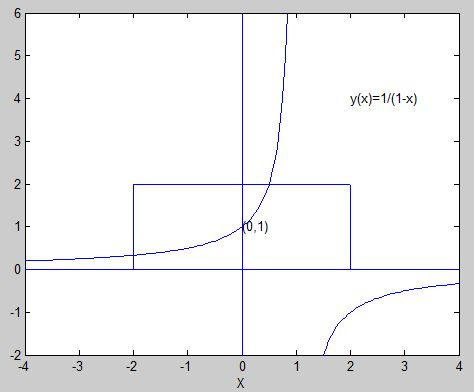
\includegraphics[width=200pt]{1-3-8}\\
图中解曲线在到达区间I的右端点之前离开矩形I
\end{note}
\subsection{一阶线性微分方程}
\begin{theorem}
  在两个系数函数P(x)与Q(x)都连续的某一区间上,求解一阶线性微分方程
  \begin{equation}
    \frac{dy}{dx}+P(x)y=Q(x)
    \label{equation 1}
  \end{equation}
  通过对\ref{equation 1}两边乘以适当的积分因子,可以得到一种标准解法,我们乘以
  \begin{equation}
   {\bf  \rho(x)=e^{\int P(x)dx}}
    \label{equation 2}
  \end{equation}
 结果为
 \begin{equation}
    e^{\int P(x)dx} \frac{dy}{dx}+P(x)e^{\int P(x)dx}y=Q(x)e^{\int P(x)dx}
    \label{equation 3}
  \end{equation}
  方程\ref{equation 3}的左边是$y(x)e^{\int P(x)dx}$的微分
  两边积分,最后求出\ref{equation 1}的通解为:
  \begin{equation}
    y(x)=e^{-\int P(x)dx}({\int {Q(x)e^{\int P(x)}dx} }+C)
  \end{equation}
\end{theorem}

\subsection{替换方法和恰当方程}
\begin{theorem}
  形如$\frac{dy}{dx}=F(ax+by+c)$ 的微分方程可以通过变换$v=ax+by+c$ 将其变化分离变量型
\end{theorem}
\subsection{恰当微分方程}
\begin{theorem}
  {\bf (恰当型判别准则)}假设在矩形开区域$R:a<x<b,c<y<d$ 上,函数M(x,y),N(x,y)连续且有连续一阶偏导数,那么微分方程
  \begin{equation}
  M(x,y)dx+N(x,y)dy=0
\end{equation}
是恰当型的充要条件是
\begin{equation}
  \frac{\partial M}{\partial y}=\frac{\partial N}{\partial x}
  \label{equation 4}
\end{equation}
在矩形R上成立.即存在R上的函数F(x,y), 满足$\frac{\partial f}{\partial x}=M,\frac{\partial f}{\partial y}=N$ 的充要条件是式\ref{equation 4}在矩形R 上成立.
\end{theorem}

\begin{note}
  一般的,为了求解恰当方程$M(x,y)dx+N(x,y)dy=0$, 我们执行以下步骤: \newline
  首先,把M(x,y) 对x 进行积分,且写成下面的形式
  $$
  F(x,y)=\int M(x,y)dx+g(y)
  $$
  然后通过$\frac{\partial F}{\partial y}=N(x,y)$ 求出g(y), 这样就得到方程的隐式解 $F(x,y)=C$
\end{note}
\begin{example}
  求解微分方程$(6xy-y^2)dx+(4y+3x^2-3xy^2)dy=0$ \newline
  解:设$M(x,y)=(6xy-y^2),N(x,y)=(4y+3x^2-3xy^2)$ 因为
  $$
  \frac{\partial M}{\partial y}=6x-3y^2=\frac{\partial N}{\partial x}
  $$
  所以方程是恰当的
  $$
  F(x,y)=\int M(x,y)dx+g(y)=\int (6xy-y^2)dx+g(y)=3x^2y-xy^3+g(y)
  $$
  然后对y进行微分,并设$\frac{\partial f}{\partial y}=N(x,y)$ 得到
  $$
  \frac{\partial f}{\partial y}=3x^2-3xy^2+g'(y)=4y+3x^2-3xy^2
  $$
  整理得到:$g'(y)=4y$, 于是$g(y)=2y^2+C_1$, 从而
  $$
  F(x,y)=3x^2y-xy^3+2y^2+C_1
  $$
  因此微分方程的隐式通解为$$3x^2y-xy^3+2y^2=C$$
\end{example}

\section{数值逼近}
\subsection{欧拉方法}
已知初值问题
\begin{equation}
  \frac{dy}{dx}=f(x,y),y(x_0)=y_0.
\end{equation}
{\bf 步长为h的欧拉方法}:应用迭代公式
\begin{equation}
  y_{n+1}=y_n+hf(x_n,y_n) ~~~(n\geqslant 0)
\end{equation}
来依次计算在各个点$x_1,x_2,x_3,\ldots,x_n$ 对真实解y=f(x)的真实值$y(x_1),y(x_2),\ldots,y(x_n)$ 的逼近值$y_1,y_2,\ldots,y_n$
\newline

\subsection{改进的欧拉方法}
已知初值问题
\begin{equation}
  \frac{dy}{dx}=f(x,y),y(x_0)=y_0.
\end{equation}
假设对步长h执行n步以后,已经得到在$x_n=x_0+nh$ 点解的真值$y(x_n)$ 逼近值$y_n$, 可应用欧拉方法来获得在点$x_{n+1}=x_n+h$ 的解的真值的一个初步估计,即称之为$u_{n+1}$ 而不是$y_{n+1}$ ,则
\begin{equation}
  u_{n+1}=y_n+hf(x_n,y_n)=y_n+hk_1. \quad k_1=f(x_n,y_n)
\end{equation}
既然$u_{n+1}\thickapprox y(x_{n+1})$, 可取$k_2=f(x_{n+1},y_{n+1})$ 作为解曲线$y=f(x)$在$x=x_{x+1}$ 点的斜率的第二个估计. \newline
当然,我们已经求出在$x=x_n$的近似斜率$k_1=f(x_n,y_n)$. 为了获得在整个区间$[x_n,x_{x+1}]$ 上解曲线平均斜率的更加精确的估计,为什么不平均这两个斜率呢? \newline 这个思想就是改进的欧拉方法的本质.
\begin{theorem}
  {\bf 算法~~~改进的欧拉方法} \newline
给定初值问题
\begin{equation}
  \frac{dy}{dx}=f(x,y),y(x_0)=y_0.
\end{equation}
步长为h的欧拉方法:应用迭代公式
$
\begin{cases}
  k_1=f(x_n,y_n) \\
  u_{n+1}=y_n+hk_1 \\
  k_2=f(x_{n+1},y_{n+1}) \\
  y_{n+1}=y_n+\frac{1}{2}h(k_1+k_2)
\end{cases}
$
\\
来依次计算$y=f(x)$在点$x_1,x_2,x_3,\ldots,x_n$的真值$y(x_1),y(x_2),\ldots,y(x_n)$ 的逼近值$y_1,y_2,\ldots,y_n$. 
\end{theorem}
\begin{note}
  改进后的欧拉方法使用的是一种称为{\bf 预测-校正}方法的一类数值技术之一. 首先计算下一个y值的预测值$u_{n+1}$ ,然后它自我校正. 这样步长为h的改进的欧拉方法\\
  由使用预测值
  \begin{equation}
    u_{n+1}=y_n+hf(x_n,y_n)
  \end{equation}
  和校正值
  \begin{equation}
    y_{n+1}=y_n+\frac{1}{2}h(f(x_n,y_n)+f(x_{n+1},y_{n+1}))
  \end{equation}
  构成.
\end{note}

\subsection{龙格-库塔方法}

\textbf{COERVIT\'E}
Une fonction f d\'efinie sur un espace norm\'e X \`a valeurs dans $ \bar{\R}:=\R\cup\{-\infty,+\infty\}$ est dite coercive sur une partie non born\'ee $ P$ de $X$ si
$$ \lim_{\mytop{\| x\| \to +\infty}{x\in P}}f(x)=+\infty $$

ou de mani\`ere plus pr\'ecise
$$
\forall\,\nu\in\R,\quad \exists\,\rho\geqslant0:\quad (x\in X ~\mbox{et}~ \|x\|\geqslant\rho) \quad\Longrightarrow\quad f(x)\geqslant\nu.
$$

Il revient au m\^eme de dire que les intersections avec P des ensembles de sous-niveau de la fonction sont born\'ees :
$$
\forall\,\nu\in\R,\qquad\{x\in P: f(x)\leqslant\nu\}~\mbox{est born\'e.}
$$
Si l'on ne sp\'ecifie pas la partie P, il est sous-entendu que P=X.

\underline{Cas d'une forme bilin\'eaire} \newline
Plus sp\'ecifiquement, une forme bilin\'eaire $a:X\times X\to\R$ est dite coercive si elle v\'erifie :
$$
\exists\,\alpha>0,\quad\forall\,x\in X:\qquad a(x,x) \geqslant \alpha\|x\|^2.
$$
Certains auteurs pr\'ef\`erent utiliser l'appellation X-elliptique pour cette derni\`ere d\'efinition. Celle-ci intervient entre autres dans le th\'eor\`eme de Lax-Milgram et la th\'eorie des op\'erateurs elliptiques, accessoirement dans la m\'ethode des \'el\'ements finis.

\underline{Lien entre les d\'efinitions}\newline
Dans le cas où a est une forme bilin\'eaire, en posant $f(u)=a(u,u)$ on a \'equivalence entre la coercivit\'e de a et celle de $f$. En effet, $\scriptstyle\lim_{\| x\|\to\infty}f(x)=+\infty $implique qu'il existe $R>0 $tel que $\scriptstyle\|x\|\geqslant R\Rightarrow f(x)\geqslant 1$. Ainsi:
$$
\left(\frac{R}{\|u\|}\right)^2a(u,u)=a\left(\frac{R}{\|u\|}u,\frac{R}{\|u\|}u\right)=f\left(\frac{R}{\|u\|}u\right)\geqslant 1
$$
et
$$
a(u,u)\geqslant\left(\frac{\|u\|}{R}\right)^2.
$$
维基百科上没有直接给出coercivit\'e的定义, 但是按照维基百科的解释, 我觉得coercivit\'e的定义是
$$
 \alpha=\left(\frac{1}{R}\right)^2
$$

\bigskip
\textbf{Application contractante}\newline
Une application contractante, ou contraction, est une application k-lipschitzienne avec $0 \geq k \le 1$
\bigskip

\textbf{Th\'eor\`eme du point fixe pour une application contractante}\newline
Soient $ E$  un espace m\'etrique complet (non vide) et $ f$  une application $ k$ -contractante de $ E$  dans $ E$ . Il existe un point fixe unique $x^*$ de f (c'est-\`a-dire un $x^*$ dans $ E$  tel que $ f(x^* ) = x^*)$ . De plus, toute suite d'\'el\'ements de E v\'erifiant la r\'ecurrence
$$x_{n+1}=f(x_n)$$
v\'erifie la majoration
$$d(x_n,x^*) \le \frac {k^n}{1-k} d(x_0,x_1)$$
donc converge vers $x^*$
\bigskip

\textbf{In\'egalit\'e de Poincar\'e}
un r\'esultat de la th\'eorie des espaces de Sobolev\\
Cette in\'egalit\'e permet de borner une fonction \`a partir d'une estimation sur ses d\'eriv\'ees et de la g\'eom\'etrie de son domaine de d\'efinition\\
L'in\'egalit\'e de Poincar\'e classique
Soit $p$, tel que $ 1 \leq p < \infinity$  et $\Omega$ un ouvert de largeur finie (born\'e dans une direction). Alors il existe une constante  $  C$  , d\'ependant uniquement de $\Omega$ et $p$, telle que, pour toute fonction $u$   de l'espace de Sobolev $W_0^{1,p(\Omega)}$
$$
\| u \|_{L^{p} (\Omega)} \leq C \| \nabla u \|_{L^{p} (\Omega)}
$$

\chapter{Variation}
\section{Fundamental lemma of variation}
\begin{theorem}
    Soit une fonction $f(x)$ est continue sur $[a,b]$,$ \forall \eta(x)$ sur $\in C^{n}[a,b]$,et $\exists m>0$,tel que $\eta^{k}(a)=\eta^{k}(b)=0 (\forall k \in [[0,n]])$ \newline
    si$ \int_{a}^{b}f(x)\eta(x)=0$ est toujours vrai, \newline
    alors, sur $[a,b],f(x)\equiv 0$ \newline
    (证明时用反证法,且需要构造$\eta(x)$为特殊的形式)
    $\exists \xi,f(\xi)>0 \Rightarrow \exists $une intervale $[a_0,b_0]$,tel que sur $[a_0,b_0],f(x)$ est positive \newline
 on peut construire $\eta(x)$ comme cidessous:
$\eta(x)=
    \left\{
      \begin{array}{ll}
        [(x-a_0)(x-b_0)]^{2n+2} & x \in [a_0,b_0] \\
        0 & sinon
      \end{array}
    \right.
    $
\end{theorem}

\textbf{Quand m=n=0}
\begin{theorem}
    Soit une fonction $f(x)$ est continue sur $[a,b]$,$ \forall \eta(x)$ sur $\in C^{0}[a,b]$,et $\exists m>0$,tel que $\eta(a)=\eta(b)=0$ \newline
    si$ \int_{a}^{b}f(x)\eta(x)=0$ est toujours vrai, \newline
    alors, sur $[a,b],f(x)\equiv 0$
\end{theorem}

\begin{theorem}
    Soit une fonction $f(x)$ est continue sur $[a,b]$,$ \forall \eta(x)$ sur $\in C^{1}[a,b]$,et $\eta(a)=\eta(b)=0$ \newline
    si$ \int_{a}^{b}f(x)\eta'(x)=0$ est toujours vrai, \newline
    alors, sur $[a,b],f(x)\equiv Constante$
\end{theorem}

\begin{theorem}
    Soit une fonction $f(x,y)$ est continue sur $D$,$ \forall \eta(x,y)$ sur $\in C^{1}[a,b]$,et 在D的边界上, $\eta(x,y)=0$\newline
    si$ \int_{a}^{b}f(x,y)\eta(x,y)=0$ est toujours vrai, \newline
    alors, sur $D,f(x,y)\equiv 0$
\end{theorem}

\section{Variational Problems with Fixed Boudaries}
\begin{definition}
  \textbf{n阶距离}:Soit deux foncitons $y(x)$ et $y_0(x)\in C^{n}[a,b]$,则这两个函数从0到n阶导数之差的绝对值中的最大值称为 $y(x)$ et $y_0(x)$在区间$[a,b]$上的n阶距离或n级距离
  $d_n[y(x),y_0(x)]=max_{0 \leqslant i \leqslant n}max_{a \leqslant x \leqslant b}|y^{(i)}(x)-y_0^{(i)}(x)|$
\end{definition}
特别地,当$n=0$时,为0阶距离;当$n=1$时,为1阶距离

\begin{definition}
\textbf{n阶领域}:函数$y_0(x)$在区间$[a,b]$上的n阶领域,记为$N_n[\delta,y_0(x)]$,表示为\newline
$N_n[\delta,y_0(x)]=\{y(x)|y(x)\in C^{n}[a,b],d_n[y(x),y_0(x)] < \delta \}$
\end{definition}
\begin{definition}
\textbf{变分}:对于任意定值$x \in [x_0,x_1]$,可取函数$y(x)$ 与另一个可取函数 $y_0(x)$ 之差$y(x)-y_0(x)$ 称为函数$y(x)$在 $y_0(x)$ 处的变分或函数的变分,记作$\delta y$,$\delta$称作变分符号或变分算子,这时有\\
$\delta y=y(x)-y_0(x)=\epsilon\eta(x)$ \newline
式中$\epsilon$为朗格朗日引进的一个小参数,但是不是x的函数,而$\eta(x)$为x的任意函数
\end{definition}
由于可取函数都通过区间的固定端点,即他们在区间的端点的值相等,且由于端点是固定的,所以在端点处的变分为零. \newline

可取函数$y(x)$ 是泛函$J[y(x)]$的宗量,故也可以这样定义变分:泛函的宗量$y(x)$与另一个宗量 $y_0(x)$ 之差$y(x)-y_0(x)$ 称为宗量$y(x)$在 $y_0(x)$ 处的变分.

\begin{attention}
函数的变分$\delta y$是x的函数.\newline
注意函数变分与函数增量$\Delta y$的区别:\newline
函数的变分是两个不同函数在x取一个定值时之差,函数发生了改变,自变量没有变;\newline
而函数的增量是由于自变量x取一个增量而使同一个函数产生的增量,函数仍是原来的函数,而自变量发生了变化
\end{attention}

\textbf{全变分}:若可取函数$y(x)$变位$y_1(x)$的同时,自变量x也取得了无穷小增量$\Delta x$,函数的增量在舍去高阶增量后,可近似写成\newline
$\Delta y=\delta y + y'(x)\Delta x$
\newline
全变分包括两部分,一部分是由于自变量变化所引起的$y'(x)\Delta x$;另一部分是由函数变化所引起的$\delta y $

$\delta y'=y'(x)-y_0'(x)=[y(x)-y_0(x)]'=(\delta y)'$
D'ou $\delta \frac{dy}{dx}=\frac{d}{dx}\delta y$
\newline
That is to say:函数导数的变分等于函数变分的倒数,换句话说,求变分与求导数这两种运算次序可以交换
\newline
上面的性质可以推广到高阶的情形
同时,我们可以推出哈密顿算子,拉普拉斯算子都可以和变分符号交换顺序

\subsection{最简泛函的变分与极值的必要条件}
Soit $F(x,y(x),y'(x))$ une fonction connue de trois variables $x,y(x),y'(x)$ sur $[x_0,x_1]$, et F 二阶连续可微,其中$y(x),y'(x)$是x的未知函数,则泛函 \newline
$$J[y(x)]=\int_{x_0}^{x_1}F(x,y(x),y'(x))dx$$
称为最简单的积分型泛函,简称最简泛函,$J[y(x)]$ 是$y(x)$的泛函,由上面的式子知,$J[y(x)]$不仅是$y(x)$的函数,而且还是$x,y'(x)$, 但是只要求出了$y(x)$, $y'(x)$也就能够求出来了, 于是泛函只是写成$J[y(x)]$的形式
\newline
最简泛函的增量也称为泛函的全变分
\begin{equation}
\begin{split}
  \Delta J=J[y_1(x)]-J[y(x)]=J[y(x)+\delta y]-J[y(x)]= \\
\int_{x_0}^{x_1}F(x,y(x)+\delta y,y'(x)+\delta y')dx-\int_{x_0}^{x_1}F(x,y(x),y'(x))dx = \\
\int_{x_0}^{x_1}[F(x,y(x)+\delta y,y'(x)+\delta y')-F(x,y(x),y'(x))]dx
 \end{split}
\end{equation}
$F(x,y(x)+\delta y,y'(x)+\delta y')-F(x,y(x),y'(x))=\overline{F_y}\delta y + \overline{F_{y'}}\delta y'$ \newline
$F(x,y(x)+\delta y,y'(x)+\delta y')-F(x,y(x),y'(x))$的线性部分是$F_y\delta y + F_{y'}\delta y'$ \\
On note $F_y\delta y + F_{y'}\delta y'$ comme $L[y,\delta y]$ \\
$L[y,\delta y]$ 是关于$\delta y$的现行泛函

\begin{definition}
若连续泛函$J[y(x)]$满足以下两个条件:\\
1. $J[y_1(x)+y_2(x)]=J[y_1(x)]+J[y_2(x)]$ \\
2. $J[cy(x)]=cJ[y(x)]$ avec c une constante\\
alors,$J[y(x)]$称为关于$y(x)$的线性泛函
\end{definition}

对称双线性泛函,双线性泛函,二次泛函\\
$$
\delta J
=\int_{x_0}^{x_1}[F_y(x,y,y')\delta y + F_{y'}(x,y,y')\delta y']dx
=\int_{x_0}^{x_1}(F_y\delta y + F_{y'}\delta y')dx
=\int_{x_0}^{x_1}(F_y\epsilon\eta + F_{y'}\epsilon\eta')dx
=\epsilon \int_{x_0}^{x_1}(F_y\eta + F_{y'}\eta')dx
$$
泛函的变分$\delta J$是泛函增量$\Delta J$的线性主要部分,即线性主部

变分记号$\delta$有下列基本运算性质\\
1.$\delta (F_1+F_2)=\delta F_1+\delta F_2$ \\
2.$\delta (F_1*F_2)=F_1\delta F_2+F_2\delta F_1$\\
3.$\delta (F^{n})=nF^{n-1}\delta F$\\
4.$\delta (\frac{F_1}{F_2})=\frac{F_2\delta F_1-F_1\delta F_2}{F_2^{2}}$\\
5.$\delta (F^{(n)})=(\delta F)^{n}$\\
6.$\delta \int_{x_0}^{x_1}F(x,y,y')dx=\int_{x_0}^{x_1}\delta F(x,y,y')dx$\\

全变分$\Delta$有下列基本运算性质\\
1.$\Delta (F_1+F_2)=\Delta F_1+\Delta F_2$ \\
2.$\Delta (F_1*F_2)=F_1\Delta F_2+F_2\Delta F_1$\\
3.$\Delta (F^{n})=nF^{n-1}\Delta F$\\
4.$\Delta (\frac{F_1}{F_2})=\frac{F_2\Delta F_1-F_1\Delta F_2}{F_2^{2}}$\\
5.$(\Delta F^{(n)})'=\Delta( F^{(n+1)})+F^{(n+1)}(\Delta x)'$ (微分与全变分的运算次序不能交换)\\
6.$\Delta \int_{x_0}^{x_1}Fdx=\delta \int_{x_0}^{x_1}Fdx + (F\delta x)|_{x_0}^{x_1}=\int_{x_0}^{x_1}(\delta F + F\frac{d}{dx}\delta x)dx $  \\性质6表明,当$\frac{d}{dx}\delta x\neq 0$时,积分与全变分的运算也不能交换顺序 \\
7.$d(\Delta x) = \Delta(dx)$
对自变量而言,全变分和微分的运算次序具有交换性

5.preuve: \\
$(\Delta F^{(n)})'=[F^{(n+1)} \Delta x + \delta (F^{(n)})]'=F^{(n+2)}\Delta x + F^{(n+1)}(\Delta x)'+ \delta (F^{(n+1)})=\Delta (F^{(n+1)}) + F^{(n+1)}(\Delta x)'$

6.preuve: \\
$$\Delta \int_{0}^{x}Fdx=\delta \int_{0}^{x}Fdx + F \Delta x$$
将上式中的积分上限x分别用$x_0,x_1$替换,可得到两个类似的关系式,然后将两个式子作差,可得到下面的关系式:
$$\Delta \int_{x_0}^{x_1}Fdx=\delta \int_{x_0}^{x_1}Fdx + (F \Delta x)|_{x_0}^{x_1}$$
and
$$\delta \int_{x_0}^{x_1}Fdx=\int_{x_0}^{x_1}\delta Fdx=\int_{x_0}^{x_1}(\Delta F -F' \Delta x)dx $$
$$(F \Delta x)|_{x_0}^{x_1}=\int_{x_0}^{x_1}d(F \Delta x)$$
将上面的两个式子代入到上面的第三个式子中得到:
$$\Delta \int_{0}^{x}Fdx=\int_{x_0}^{x_1}(\Delta F -F' \Delta x)dx +\int_{x_0}^{x_1}d(F \Delta x)=\int_{x_0}^{x_1}[\Delta F + F (\Delta x)']dx$$
\subsection{最简泛函的欧拉方程}
\begin{theorem}
使最简泛函
$$J[y(x)]=\int_{x_0}^{x_1}F(x,y(x),y'(x))dx$$
取极值且满足固定边界条件
$$
y(x_0)=y_0,y(x_1)=y_1
$$
的极值曲线$y=y(x)$应满足\textbf{必要条件}(欧拉方程)
$$
F_y - \frac{d}{dx}F_{y'} =0
$$
的解,式中$F$是$x,y,y'$的已知函数并有二阶连续偏导数
取得极值 $\Leftrightarrow \delta J = \int_{x_0}^{x_1}(F_y \delta y + F_{y'} \delta y')dx=0$
\end{theorem}

\subsection{依赖于多个一元函数的变分问题}
\begin{theorem}
使泛函$$J[y(x),z(x)]=\int_{x_0}^{x_1}F(x,y,y',z,z')dx$$取得极值且满足固定边界条件
$$
y(x_0)=y_0,y(x_1)=y_1,z(x_0)=z_0,z(x_1)=z_1
$$
的极值曲线$y=y(x),z=z(x)$必满足欧拉方程组
$$
\left\{
  \begin{array}{ll}
    F_y - \frac{d}{dx}F_{y'}=0 & \\
    F_z - \frac{d}{dx}F_{z'}=0 &
  \end{array}
\right.
$$
\end{theorem}

\begin{corollary}
对于含有n个未知数$y_1(x),y_2(x) ,\ldots , y_n(x)$,使泛函
$$J[y_1,y_2 ,\ldots , y_n]=\int_{x_0}^{x_1}F(x,y_1,y_2 ,\ldots , y_n,y_1',y_2' ,\ldots , y_n')dx$$
取得极值并且满足边界条件
$$y_i(x_0)=y_{i0},y_i(x_1)=y_{i1} ~(i=1,2,\dots,n)$$
的极值曲线$y_i=y_i(x)~ (i=1,2,\dots,n)$比满足欧拉方程组
$$F_{y_i} -  \frac{d}{dx}F_{y_i'}=0 ~(i=1,2,\dots,n)$$
\end{corollary}

\subsection{依赖于高阶导数的变分问题}
\begin{theorem}
使泛函
$$J[y(x)]=\int_{x_0}^{x_1}F(x,y,y',y'')dx$$
取极值且满足固定边界条件
$$
y(x_0)=y_0,y(x_1)=y_1,y'(x_0)=y_0',y'(x_1)=y_1'
$$
的极值曲线$y=y(x)$必满足微分方程
$$F_y - \frac{d}{dx}F_y' + \frac{d^2}{dx^2}F_{y''} = 0 $$
\end{theorem}

\begin{corollary}
使依赖于未知函数$y(x)$的n阶导数的泛函
$$J[y]=\int_{x_0}^{x_1}F(x,y,y',y'', \ldots , y^{(n)})dx$$
取极值且满足固定边界条件
$$
y^{(k)}(x_0)=y_0^{(k)}, y^{(k)}(x_1)=y_1^{(k)} ~ (k= 0,1,\ldots , n-1)
$$
的极值曲线$y=y(x)$必满足欧拉-泊松方程
$$F_y - \frac{d}{dx}F_{y'} + \frac{d^2}{dx^2}F_{y''} - \dots + (-1)^{n}\frac{d^n}{dx^n}F_{y^{(n)}}=0  $$
式中F具有n+1阶连续导数,y具有2n阶连续导数,这是一个2n阶微分方程,它的通解中含有2n个特定常数,可由2n个边界来确定
\end{corollary}

\begin{corollary}
使依赖于两个未知函数$y(x)$的m阶导数,$z(x)$的n阶导数的泛函
$$J[y(x),z(x)]=\int_{x_0}^{x_1}F(x,y,y',y'', \ldots , y^{(m)},z,z',z'', \ldots , z^{(n)})dx$$
取极值且满足固定边界条件
$$
y^{(k)}(x_0)=y_0^{(k)}, y^{(k)}(x_1)=y_1^{(k)} ~ (k= 0,1,\ldots , m-1)
$$
$$
z^{(k)}(x_0)=z_0^{(k)}, z^{(k)}(x_1)=z_1^{(k)} ~ (k= 0,1,\ldots , n-1)
$$
的极值曲线$y=y(x),z=z(x)$必满足欧拉-泊松方程
$$
\left\{
  \begin{array}{ll}
    F_y - \frac{d}{dx}F_{y'} + \frac{d^2}{dx^2}F_{y''} - \dots + (-1)^{n}\frac{d^n}{dx^n}F_{y^{(n)}}=0 &\\
    F_z - \frac{d}{dx}F_{z'} + \frac{d^2}{dx^2}F_{z''} - \dots + (-1)^{n}\frac{d^n}{dx^n}F_{z^{(n)}}=0   &
  \end{array}
\right.
$$
式中F具有n+1阶连续导数,y,z具有2n阶连续导数
\\
当然我们还可以推论到更多个未知函数的情况
\end{corollary}

\subsection{依赖于多元函数的变分问题}
\begin{theorem}
设D是平面区域,$(x,y) \in D ,u(x,y) \in C^2(D)$,使泛函
$$
J[u(x,y)]=\int\int_{D}F(x,y,u_x,u_y)dxdy
$$
取极值且在区域D的边界线L上取已知的极值函数$u=u(x,y)$必须满足偏微分方程
$$
F_u -\frac{\partial}{\partial x}F_{u_x}-\frac{\partial}{\partial y}F_{u_y} = 0
$$
这个方程称为奥斯特罗格拉茨基方程,简称奥氏方程,有时也称之为欧拉方程
\end{theorem}

\begin{corollary}
设D是平面区域,$(x,y) \in D ,u(x,y) \in C^4(D),F(x,y,u,u_x,u_y,u_{xx},u_{xy},u_{yy}) \in C^3$,则泛函
$$
J[u(x,y)]=\int\int_{D}F(x,y,u,u_x,u_y,u_{xx},u_{xy},u_{yy})dxdy
$$
的奥氏方程为
$$
F_u -\frac{\partial}{\partial x}F_{u_x}-\frac{\partial}{\partial y}F_{u_y}+ \frac{\partial^2}{\partial x^2}F_{u_{xx}} + \frac{\partial^2}{\partial x \partial y}F_{u_{xy}} + \frac{\partial^2}{\partial y^2}F_{u_{yy}} = 0
$$
\end{corollary}

\begin{corollary}
设D是平面区域,$(x,y) \in D, u(x,y) \in C^{2n}(D),F \in C^{n+1}(D)$,则泛函
$$
J[u(x,y)]=\int\int_{D}F(x,t,u,u_x,u_y,u_{xx},u_{yy}, \ldots , u_{\underbrace{xx \dots x}_{n}},u_{\underbrace{yy \dots y}_{n}})dxdy
$$
的奥氏方程为
$$
\begin{array}{c}
   F_u -\frac{\partial}{\partial x}F_{u_x}-\frac{\partial}{\partial y}F_{u_y}+ \frac{\partial^2}{\partial x^2}F_{u_{xx}} + \frac{\partial^2}{\partial x \partial y}F_{u_{xy}} + \frac{\partial^2}{\partial y^2}F_{u_{yy}} + \dots +  \\
 \\
   (-1)^n (
\frac{\partial^n }{\partial x^n}F_{u_{\underbrace{xx \dots x}_{n}}}+
\frac{\partial^n }{\partial x^{n-1}\partial y}F_{u_{\underbrace{xx \dots y}_{n-1}}}+
\dots+
\frac{\partial^n }{\partial y^n}F_{u_{\underbrace{yy \dots y}_{n}}})
= 0
\end{array}
$$
\end{corollary}

\begin{corollary}
设D是平面区域,$(x,y) \in D ,u(x,y) \in C^2(D),v(x,y) \in C^2(D)$,使泛函
$$
J[u(x,y),v(x,y)]=\int\int_{D}F(x,y,,u,v,u_x,,v_x,u_y,v_y)dxdy
$$
的奥氏方程组为
$$
\left\{
  \begin{array}{ll}
   F_u -\frac{\partial}{\partial x}F_{u_x}-\frac{\partial}{\partial y}F_{u_y} = 0 \\
   F_v -\frac{\partial}{\partial x}F_{v_x}-\frac{\partial}{\partial y}F_{v_y} = 0
  \end{array}
\right.
$$
\end{corollary}

\section{可动边界的变分问题}
\subsection{最简泛函的变分问题}
设泛函
\begin{equation}
  J[y(x)]=\int_{x_0}^{x_1}F(x,y,y')dx
\label{equation.function.simple-general}
\end{equation}

其可取曲线$y = y(x) \in C^2$类函数,且两个端点$A(x_0,y_0),B(x_1,y_1)$ 分别在两个给定的$C^2$类函数,此时称为可动边界的最简泛函或待定边界的最简泛函。\\

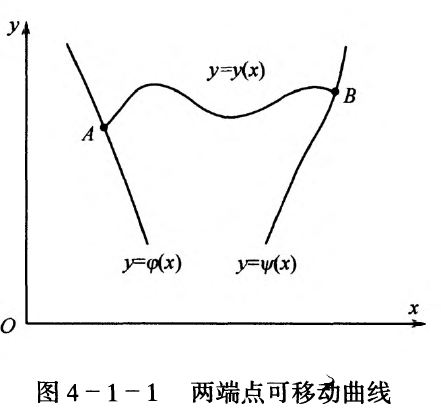
\includegraphics[width=0.5\textwidth]{limit-move}\\

若函数$y=y(x)$能在可动边界的容许函数类中使泛函(\ref{equation.function.simple-general})取得极值,
那么必能在固定边界的容许函数类中使泛函取得极值,这是因为可动边界泛函的容许曲线类的范围扩大了,当然包含了固定边界泛函的容许曲线,
而在固定边界情况下使泛函取得极值的函数必须满足欧拉方程,所以函数(\ref{equation.function.simple-general})在可动边界情况下也应当满足欧拉方程
$$
F_y - \frac{d}{dx}F_{y'} =0
$$
欧拉方程的解含有两个任意常数,它的一般解形式为
$$y=y(x,c_1,c_2)$$
在端点固定的情况下,这两个常数可以解出来,在可动边界条件下,他们都是$x_0,x_1$的函数,确定他们的条件就是泛函取得极值的必要条件$\delta J=0$

如图所示,A点固定,B点可以变动,当B点从$(x_1,y_1)$移动到$(x_1+\delta x_1,y_1+\delta y_1)$时,泛函$ J[y(x)]$的增量
\begin{equation}
     \begin{split}
         & \Delta J=\int_{x_0}^{x_1+\delta x_1}F(x,y+\delta y,y'+\delta y')dx-\int_{x_0}^{x_1}F(x,y,y')dx\\
         & =\int_{x_0}^{x_1+\delta x_1}F(x,y+\delta y,y'+\delta y')dx+\int_{x_0}^{x_1}[F(x,y+\delta y,y'+\delta y')-F(x,y,y')]dx
     \end{split}
\end{equation}
略去高阶无穷小量后剩下一阶变分为
\begin{equation}
\begin{split}
     &  \delta J=\int_{x_0}^{x_1}(F_y - \frac{d}{dx}F_{y'} )\delta y dx + F|_{x=x_1}\delta x_1 + F_{y'}|_{x=x_1}[\delta y_1 - y'(x_1)\delta x_1] \\
    & =\int_{x_0}^{x_1}(F_y - \frac{d}{dx}F_{y'} )\delta y dx + (F-y'F_{y'})|_{x=x_1}\delta x_1 +F_{y'}|_{x=x_1}\delta y_1
\end{split}
\end{equation}
因为泛函的极值只能在极值曲线上取得,所以
$F_y - \frac{d}{dx}F_{y'} \equiv0$
上式化为
\begin{equation}
     \delta J=(F-y'F_{y'})|_{x=x_1}\delta x_1 +F_{y'}|_{x=x_1}\delta y_1
\end{equation}
再由条件$\delta J=0$得
\begin{equation}
     (F-y'F_{y'})|_{x=x_1}\delta x_1 +F_{y'}|_{x=x_1}\delta y_1=0
     \label{equation.result.general}
\end{equation}
如果$\delta x_1,\delta y_1$相互无关,则由(\ref{equation.result.general})得到
\begin{equation}
(F-y'F_{y'})|_{x=x_1}=0
\label{equation.result.unrelated.1}
\end{equation}
\begin{equation}
F_{y'}=0
\label{equation.result.unrelated.2}
\end{equation}
当我们把(\ref{equation.result.unrelated.2})代入(\ref{equation.result.unrelated.1})我们得到$F_y=0$,因此我们有必要考虑$\delta x_1,\delta y_1$相关
\begin{theorem}
设泛函$J[y(x)]=\int_{x_0}^{x_1}F(x,y,y')dx$的极值曲线$y=y(x)$一端固定,另一端在直线$x=x_1$上待定,则可动的一端必满足自然边界条件(\ref{equation.result.unrelated.2})
若极值曲线$y=y(x)$的端点在已知直线$y=\psi(x)$上待定,则变分$\delta x_1,\delta y_1$相关
\end{theorem}

\begin{theorem}
设泛函$J[y(x)]=\int_{x_0}^{x_1}F(x,y,y')dx$的极值曲线$y=y(x)$左端固定,右端点在已知直线$y=\psi(x)$上待定,则右端点在$x=x_1$处必满足
\begin{equation}
[F + (\psi' - y')F_{y'}]|_{x=x_1}=0
\end{equation}
\end{theorem}
\begin{proof}
 对已知曲线$y=\psi(x)$取变分,得到 $\delta y=\psi'(x)\delta x$,在右端点处,$\delta y_1=\psi'(x_1)\delta x_1$ \\
将之代入到(\ref{equation.result.general})可以得到
$$
[F + (\psi' - y')F_{y'}]|_{x=x_1}\delta x_1=0
$$
又因为$\delta x_1$是任意的,所以可以得到
$[F + (\psi' - y')F_{y'}]|_{x=x_1}=0$
\end{proof}
上式建立了极值曲线$y = y ( x )$与已知曲线:$y = \psi(x)$在交点B 处的$y'$与$\psi'$两斜率
之间的关系,这样的关系称为横截(性)条件、贯截条件或斜截条件。这两条曲线较小的那个交角称
为斜截角。

\begin{theorem}
\label{theorem.limit.two}
设泛函$J[y(x)]=\int_{x_0}^{x_1}F(x,y,y')dx$的极值曲线$y=y(x)$左端固定在直线$y=\varphi(x)$,右端点在已知直线$y=\psi(x)$上待定,\\
则左端点在$x=x_0$处必满足
\begin{equation}
[F + (\varphi' - y')F_{y'}]|_{x=x_0}=0
\end{equation}
则右端点在$x=x_1$处必满足
\begin{equation}
[F + (\psi' - y')F_{y'}]|_{x=x_1}=0
\end{equation}
\end{theorem}
求平面上两条曲线的最短距离是定理(\ref{theorem.limit.two})的一个常见的应用,在此情况下,该定理可以化为更具体的形式.该问题归结为求泛函
$$J[y]=\int_{x_0}^{x_1}\sqrt{1+y'^2}dx$$的极小值

\subsection{含有多个函数的泛函的变分问题}
设空间曲线
\begin{equation}
J[y(x),z(x)]=\int_{x_0}^{x_1}F(x,y,z,y',z')dx
\label{equation.general.space}
\end{equation}
式中$y,z \in C^2[x_0,x_1],F \in C^2$,容许曲线$y=y(x),z=z(x)$在左端点
$A(x_0,y_0,z_0)$固定,右端点 $B(x_1,y_1,z_1)$待定
泛函的(\ref{equation.general.space})的变分可模仿上节的方法进行
\begin{equation}
\begin{array}{c}
  \Delta J=\int_{x_0}^{x_1+\delta x_1}F(x,y+\delta y,z+\delta z,y'+\delta y',z'+\delta z')dx-\int_{x_0}^{x_1}F(x,y,z,y',z')dx\\
\\
  = \int_{x_1}^{x_1+\delta x_1}F(x,y+\delta y,z+\delta z,y'+\delta y',z'+\delta z')dx +\\
\\
\int_{x_0}^{x_1}[F(x,y+\delta y,z+\delta z,y'+\delta y',z'+\delta z')-F(x,y,z,y',z')]dx
\end{array}
\end{equation}
它的线性主部
\begin{equation}
 \delta J=F|_{x=x_1}\delta x_1 +F_{y'}\delta y|_{x=x_1} +F_{z'}\delta z|_{x=x_1} +
 \int_{x_0}^{x_1}[(F_y - \frac{d}{dx}F_{y'}) \delta y +(F_z -\frac{d}{dx}F_{z'} )\delta z]dx
\end{equation}
因为泛函$J[y,z]$的极值只能在极值曲线上取得,故必须满足欧拉方程组
$$
\left\{
  \begin{array}{ll}
    F_y - \frac{d}{dx}F_{y'}=0 & \\
    F_z - \frac{d}{dx}F_{z'}=0 &
  \end{array}
\right.
$$
这个方程组的通解中含有四个任意常数,由于B点可以变动,又多了一个未知量$x_1$,为了使泛函(\ref{equation.general.space})有唯一一组解,就需要确定五个常数.因为A点固定,由$y(x_0)=y_0,z(x_0)=z_0$可以定出两个常数,其余三个常数可根据泛函的极值条件$\delta J=0$确定
将欧拉方程组代入得到
\begin{equation}
 \delta J=F|_{x=x_1}\delta x_1 +F_{y'}\delta y|_{x=x_1} +F_{z'}\delta z|_{x=x_1}=0
\end{equation}
根据上一节的讨论有
\begin{equation}
 \delta y|_{x=x_1}=\delta y_1 - y'(x_1)\delta x_1, \delta z|_{x=x_1}=\delta z_1 - z'(x_1)\delta x_1
\end{equation}
代入上式得
\begin{equation}
 \delta J=(F - y'F_{y'} - z'F_{z'})|_{x=x_1} + F_{y'}|_{x=x_1}\delta y_1 + F_{z'}|_{x=x_1}\delta z_1=0
\label{equation.cases}
\end{equation}
式中的$\delta x_1.\delta y_1,\delta z_1$是任意的,即B点可以按照任意方式变动.根据$y_1,z_1与x_1$之间的关系,可分四种情况来讨论
\\
(1)若变分$\delta x_1.\delta y_1,\delta z_1$相互无关,则可以得到
$$
\left\{
  \begin{array}{ll}
     & (F - y'F_{y'} - z'F_{z'})|_{x=x_1}=0 \\
     &  F_{y'}|_{x=x_1}=0\\
     & F_{z'}|_{x=x_1}=0
  \end{array}
\right.
$$
此时,如果把后两式代入第一个式子中,则有$F|_{x=x_1}=0$,即泛函的被积函数为零,一般来说这样的变分问题无意义
\\
(2)若边界点$B(x_1,y_1,z_1)$沿着某一曲线
$y_1=\varphi(x_1),z_1=\psi(x_1)$
变动时,则
$\delta y_1=\varphi'(x_1)\delta x_1,\delta z_1=\psi'(x_1)\delta x_1$
将他们代入(\ref{equation.cases})并整理,同时注意到$\delta x_1$是任意的,得
\begin{equation}
 [F + (\varphi' - y')F_{y'} + (\psi' -z')F_{z'}]|_{x=x_1}=0
\label{equation.case2}
\end{equation}
式(\ref{equation.case2})称为泛函$J[y,z]$的极值曲线与端点曲线及极值问题的横截条件,它与方程
$y_1=\varphi(x_1),z_1=\phi(x_1)$
一起就能确定欧拉方程组的通解中的任意常数
\\
(3)若边界点$B(x_1,y_1,z_1)$沿着某一曲面$\phi(x_1,y_1,z_1)=0$变动,则
\begin{equation}
 \phi_{x_1}\delta x_1+
 \phi_{y_1}\delta y_1+
 \phi_{z_1}\delta z_1=0
\end{equation}
设$\phi_{x_1}\neq 0$,则可解出$\delta z_1$
代入(\ref{equation.cases})得
\begin{equation}
(F - y'F_{y'} - z'F_{z'} - F_{z'}\frac{\phi_x}{\phi_z})|_{x=x_1} \delta x_1 +
(F_{z'} -F_{z'}\frac{\phi_y}{\phi_z})|_{x=x_1} \delta y_1  )
=0
\end{equation}
由于$\delta x_1,\delta y_1$是任意的,故边界条件为
\begin{equation}
\left\{
  \begin{array}{lll}
     & (F - y'F_{y'} - z'F_{z'} - F_{z'}\frac{\phi_x}{\phi_z})|_{x=x_1} =0 \\
&\\
    & (F_{z'} -F_{z'}\frac{\phi_y}{\phi_z})|_{x=x_1} =0
  \end{array}
\right.
\label{equation.case3}
\end{equation}
将(\ref{equation.case3})与曲面方程$\phi(x_1,y_1,z_1)=0$联立,即可求出极值曲线
\\
(4)若边界点$B(x_1,y_1,z_1)$可在空间平面$x=x_1$上变动,则$\delta x_1=0$,$\delta y_1,\delta z_1$可任意取值,自然边界条件为
\begin{equation}
F_{y'}|_{x=x_1}=0,
F_{z'}|_{x=x_1}=0
\end{equation}

\subsection{含有高阶导数的泛函的变分问题}
设泛函
\begin{equation}
 J[y(x)]=\int_{x_0}^{x_1}F(x,y,y',y'')dx
\end{equation}
式中$y \in C^2[x_0,x_1],F \in C^3$,容许曲线$y=y(x)$在左端点$A(x_0,y_0)$固定,在右端点$B(x_1,y_1)$可变,泛函的极值曲线必满足欧拉-泊松方程
$$F_y - \frac{d}{dx}F_{y'} + \frac{d^2}{dx^2}F_{y''}=0  $$
通常情况下,上式是一个四阶微分方程,其通解含有四个任意常数,右端点B可变,所以$x_1$也待定,总共五个任意常数,左端点A固定可以确定两个,
剩余的三个任意常数必须通过泛函取得极值的必要条件$\delta J=0$得到
这里还是就一般情况进行讨论,先计算泛函的增量$\Delta J$,然后再分离出线性主部$\delta J$
泛函的增量
\begin{equation}
 \begin{split}
 \Delta J = & \int_{x_0}^{x_1+\delta x_1}F(x,y+\delta y,y'+\delta y',y''+\delta y'')dx- \int_{x_0}^{x_1}F(x,y,y',y'')dx \\
              &  =\int_{x_1}^{x_1+\delta x_1}F(x,y+\delta y,y'+\delta y',y''+\delta y'')dx + \\
               & \int_{x_0}^{x_1}[F(x,y+\delta y,y'+\delta y',y''+\delta y'') -F(x,y,y',y'') ]dx
 \end{split}
\end{equation}
最后化简得
\begin{equation}
\begin{split}
 \delta J = & [F - y'(F_{y'}-\frac{d}{dx}F_{y''}) - y''F_{y''}]|_{x=x_1} \delta x_1 + \\
 & (F_{y'}-\frac{d}{dx}F_{y''})|_{x=x_1}\delta y_1 + F_{y''}\delta y_1 =0
\end{split}
\end{equation}
如果上式中$\delta x , \delta y_1, \delta y'_1$之间是相互独立的,则他们的系数在点$x=x_1$处应该为零,及自然边界条件
\begin{equation}
\left\{
  \begin{array}{ll}
[F - y'(F_{y'}-\frac{d}{dx}F_{y''}) - y''F_{y''}]|_{x=x_1}=0 \\
(F_{y'}-\frac{d}{dx}F_{y''})|_{x=x_1}=0\\
F_{y''}=0
  \end{array}
\right.
\end{equation}
同样,若把后两式代入第一式中,仍可得到$F|_{x=x_1}=0$,一般情况下,这样的变分问题无意义.若使变分问题有意义,应在可动的右端点给出一个已知条件。于
是,三个式子中的后两个条件、右端点给出的一个已知条件加上固定端点的两个条件,就可以确 定极值曲线
$y=y(x,c_1,c_2,c_3,c_4)$中的五个待定常量
中的五个待定常量。
\begin{theorem}
 高阶泛函在某一端点固定$y(x_0)=y_0,y'(x_0)=y'_0$,另一端点$(x_1,y_1)$在给定一个已知条件下,其极值曲线$y=y(x)$在端点处
必满足自然边界条件的后两个条件
\end{theorem}

\subsection{单侧变分问题}
如果变分问题中的极值函数服从于某个不等式,则把受有这种不等式约束的变分问题成为单侧变分问题.考虑最简泛函
\begin{equation}
 J[y(x)]=\int_{x_0}^{x_1}F(x,y,y')dx
\end{equation}
在不等式
\begin{equation}
 y(x) \geqslant \varphi(x)
\end{equation}
约束条件下的极值条件,其中$\varphi(x)$是给定的具有连续倒数的函数
\begin{theorem}
 极值曲线$y=y(x)$与曲线$y=\varphi(x)$在M,N两点相切
\end{theorem}

\section{条件极值的变分问题}
\subsection{完整约束的变分问题}
本节主要研究
\begin{equation}
J[y]=\int_{x_0}^{x_1}F(x,y_1,y_2, \cdots , y_n,y_1',y_2', \cdots , y_n')dx
\label{equation.fonctionGenerale}
\end{equation}
在约束条件
\begin{equation}
\varphi_i(x,y_1,y_2, \cdots , y_n)=0 ~ (i=0,1,2,\cdots ,m;m<n)
\label{equation.condition.constraint}
\end{equation}
及边界条件
\begin{equation}
y_j(x_0)=y_{jo},y_j(x_1)=y_{j1}~ (j=1,2,\cdots ,n)
\label{equation.condition.limit}
\end{equation}
的极值问题
\begin{theorem}
拉格朗日定理:在完整约束~\ref{equation.condition.constraint}和边界约束~\ref{equation.condition.limit}下使目标泛函~\ref{equation.fonctionGenerale}取得极值,则存在待定函数$\lambda_i(x)$,使得函数$y_1,y_2,\cdots,y_n$满足由下列泛函
\begin{equation}
J^{*}[y]=\int_{x_0}^{x_1}[F+\sum_{i=1}^{m}\lambda_i(x)\varphi_i]dx=\int_{x_0}^{x_1}Hdx
\label{equation.fonctionGenerale.help}
\end{equation}
所给出的欧拉方程组
$$H_{y_j} - \frac{d}{dx}H_{y_{j}'}=0 ~ (j=1,2,\cdots,n)$$
方程~\ref{equation.fonctionGenerale.help}称为辅助泛函
在对~\ref{equation.fonctionGenerale.help}进行变分运算时,应把$y_i,y_i',\lambda_i(x)$都看作是泛函$J^{*}[y]$的独立函数
\end{theorem}
微分,等周等其他约束也可以采用拉格朗日乘数法解决

\section{参数形式的变分问题}
正n次齐次函数
具有
$$
f(x,y,k\dot{x},k\dot{y})=k^nf(x,y,\dot{x},\dot{y})
$$
性质的函数称为关于$\dot{x},\dot{y}$的n次齐次函数\\
如果k是正数,则这样的函数称为关于$\dot{x},\dot{y}$的正n次齐次函数

\section{力学中的变分原理及其应用}
$$
\text{力学原理}
\left\{
	\begin{array}{ll}
	 \text{非变分的}
	 	\left\{
			\begin{array}{ll}
                    \text{微分的(如达朗贝尔原理)}\\
                    \text{积分的(如能量守恒原理)}
			\end{array}
			\right.  \\
	 \text{变分的}
	 	\left\{
			\begin{array}{ll}
                    \text{微分的(如虚位移原理)}\\
                    \text{积分的(如哈密顿原理)}
			\end{array}
			\right.
	\end{array}
	\right.
$$

\begin{equation}
\text{应变与位移的关系}
\left\{
	\begin{array}{ll}
	\varepsilon_x = \frac{\partial u}{\partial x} \\
	\varepsilon_y = \frac{\partial v}{\partial y} \\
	\varepsilon_z = \frac{\partial w}{\partial z} \\
    \gamma_{xy} = \gamma_{yx} = \frac{\partial u}{\partial y}+ \frac{\partial v}{\partial x}\\
    \gamma_{yz} = \gamma_{zy} = \frac{\partial v}{\partial z}+ \frac{\partial w}{\partial y}\\
    \gamma_{zx} = \gamma_{xz} = \frac{\partial w}{\partial x}+ \frac{\partial u}{\partial z}\\
	\end{array}
	\right.
\label{equation.cauchy}
\end{equation}

\begin{equation}
\text{应变张量}
[\varepsilon_{ij}]=
\left[
  \begin{array}{ccc}
  \varepsilon_{xx} & \varepsilon_{xy} & \varepsilon_{xz} \\
  \varepsilon_{yx} & \varepsilon_{yy} & \varepsilon_{yz} \\
  \varepsilon_{zz} & \varepsilon_{zz} & \varepsilon_{zz}
  \end{array}
\right]
=
\left[
  \begin{array}{ccc}
  \varepsilon_{x} & \frac{1}{2}\gamma_{xy} & \frac{1}{2}\gamma_{xz} \\
  \frac{1}{2}\gamma_{yx} & \varepsilon_{y} & \frac{1}{2}\gamma_{yz} \\
  \frac{1}{2}\gamma_{zz} & \frac{1}{2}\gamma_{zz} & \varepsilon_{z}
  \end{array}
\right]
\end{equation}

\begin{equation}
 \varepsilon_{ij}=\frac{1}{2}(u_{i,j}+u_{j,i})
\end{equation}

由柯西方程(\ref{equation.cauchy})可得
\begin{equation}
  \left\{
	\begin{array}{ll}
	\frac{\partial^2 \varepsilon_x }{\partial y^2} + \frac{\partial^2 \varepsilon_y }{\partial x^2} = \frac{\partial^2 \gamma_{xy}}{\partial x\partial y} , \frac{\partial}{\partial x}(- \frac{\partial \gamma_{yz}}{\partial x} +\frac{\partial \gamma_{zx}}{\partial y} +\frac{\partial \gamma_{xy}}{\partial z} ) = 2 \frac{\partial^2 \varepsilon_x}{\partial y\partial z}
	\\\\
	\frac{\partial^2 \varepsilon_y }{\partial z^2} + \frac{\partial^2 \varepsilon_z }{\partial y^2} = \frac{\partial^2 \gamma_{yz}}{\partial y\partial z} , \frac{\partial}{\partial y}(- \frac{\partial \gamma_{zx}}{\partial y} +\frac{\partial \gamma_{xy}}{\partial z} +\frac{\partial \gamma_{yz}}{\partial x} ) = 2 \frac{\partial^2 \varepsilon_y}{\partial z\partial x}
\\\\
	\frac{\partial^2 \varepsilon_z }{\partial x^2} + \frac{\partial^2 \varepsilon_x }{\partial z^2} = \frac{\partial^2 \gamma_{zx}}{\partial z\partial x} , \frac{\partial}{\partial z}(- \frac{\partial \gamma_{xy}}{\partial z} +\frac{\partial \gamma_{yz}}{\partial x} +\frac{\partial \gamma_{zx}}{\partial y} ) = 2 \frac{\partial^2 \varepsilon_z}{\partial x\partial y}
	\end{array}
	\right.
\label{equation.compatibility}
\end{equation}
(\ref{equation.compatibility})称为应变协调方程或相容性方程\\

\textbf{平衡方程—六个应力分量的三个平衡方程}
\textbf{几何方程—6个应变分量与3个位移分量}

由六个应变分量求解三个位移分量,其方程个数多于未知数个数,方程组要么矛盾,要么相关。由于变形连续,弹性体任意一点的变形必须受到其相邻单元体变形的约束。
——应变协调方程—反映应变分量之间的关系
六个应变分量必须满足一定的条件\\

从几何方程中消去位移分量,第一式和第二式分别对y和 x求二阶偏导数,然后相加,可得:
$$
\frac{\partial^2 \varepsilon_x }{\partial y^2} + \frac{\partial^2 \varepsilon_y }{\partial x^2} =
\frac{\partial^2}{\partial x \partial y}(\frac{\partial v}{\partial x}+\frac{\partial u}{\partial y})=
\frac{\partial^2 \gamma_{xy}}{\partial x\partial y}
$$

将几何方程的四,五,六式分别对z,x,y,求一阶偏导数,前后两式相加并减去中间一式,则
$$
- \frac{\partial \gamma_{yz}}{\partial x} +\frac{\partial \gamma_{zx}}{\partial y} +\frac{\partial \gamma_{xy}}{\partial z}
=2 \frac{\partial ^2 u}{\partial y \partial z}
$$
对x求一阶偏导数,则
$$
\frac{\partial}{\partial x}(- \frac{\partial \gamma_{yz}}{\partial x} +\frac{\partial \gamma_{zx}}{\partial y} +\frac{\partial \gamma_{xy}}{\partial z} ) = 2 \frac{\partial^2 \varepsilon_x}{\partial y\partial z}
$$
分别轮换x,y,z,则可得如下六个关系式

\textbf{变形协调方程的数学意义}
使3个位移为未知函数的六个几何方程不相矛盾

\textbf{变形协调方程的物理意义}
物体变形后每一单元体都发生形状改变,如变形不满足一定的关系,变形后的单元体将不能重新组合成连续体,其间将产生缝隙或嵌入现象。
为使变形后的物体保持连续体,应变分量必须满足一定的关系。

\begin{equation}
\text{应力张量}
\sigma=
[\sigma_{ij}]=
\left[
  \begin{array}{ccc}
  \sigma_{11} & \sigma_{12} & \sigma_{13} \\
  \sigma_{21} & \sigma_{22} & \sigma_{23} \\
  \sigma_{31} & \sigma_{32} & \sigma_{33}
  \end{array}
\right]
=
\left[
  \begin{array}{ccc}
  \sigma_{xx} & \sigma_{xy} & \sigma_{xz} \\
  \sigma_{yx} & \sigma_{yy} & \sigma_{yz} \\
  \sigma_{zz} & \sigma_{zz} & \sigma_{zz}
  \end{array}
\right]
=
\left[
  \begin{array}{ccc}
  \sigma_{x} & \tau_{xy} & \tau_{xz} \\
  \tau_{yx} & \sigma_{y} & \tau_{yz} \\
  \tau_{zz} & \tau_{zz} & \sigma_{z}
  \end{array}
\right]
\end{equation}
应力张量是对称张量

\subsection{常用的应变能公式}
设L为直杆长度,A为直杆面积,E为直杆材料弹性模量,在直杆为线弹性的情况下,根据材料力学的理论,下列应变能公式成立\\
\textbf{拉伸(伸缩)应变能}
\begin{equation}
 U=\frac{P\Delta L}{2}=\frac{\sigma \varepsilon}{2}AL=\frac{EAL\varepsilon^2}{2}=\frac{P^2L}{2EA}
\end{equation}
\begin{equation}
 U=\frac{1}{2}\int_{0}^{L}\frac{P^2}{EA}dx=\frac{1}{2}\int_{0}^{L}EA(\frac{du}{dx})^2dx
\end{equation}
式中,P为轴向力,$\Delta L$为直杆变形量,u为相应x长度轴向位移量,$\sigma,\varepsilon$分别为直杆的应力和应变

\textbf{弯曲应变能}
\begin{equation}
 U=\frac{1}{2}\int_{0}^{L}\frac{M^2}{EI}dx=\frac{1}{2}\int_{0}^{L}EIk^2dx
\end{equation}
式中,M为弯矩,k是曲率,EI为横截面抗弯刚度,I为截面惯性矩\\
根据高等数学,曲率的表达式为
\begin{equation}
 k=|\frac{y''}{(1+y')^{\frac{3}{2}}}|
\end{equation}
在小变形的情况下,$y''=0$,于是弯曲应变能可改写成
\begin{equation}
 U=\frac{1}{2}\int_{0}^{L}\frac{M^2}{EI}dx=\frac{1}{2}\int_{0}^{L}EIy''^2dx
\end{equation}

\textbf{剪切应变能}
\begin{equation}
 U=\frac{1}{2}\int_{0}^{L}\frac{kQ^2}{GA}dx=\frac{1}{2}\int_{0}^{L}\frac{GA\gamma^2}{k}dx
\end{equation}
式中,Q为剪力,$\gamma$为剪应变,k为截面剪应力分布有关的系数,$GA/k$为截面抗剪刚度

\textbf{园轴扭转应变能}
\begin{equation}
 U=\frac{M_t^2 L}{2GJ_p}=\frac{GJ_p\phi^2}{2L}
\end{equation}
\begin{equation}
 U=\frac{1}{2}\int_{0}^{L}\frac{M_t^2}{GJ_p}dx=\frac{1}{2}\int_{0}^{L}GJ_p(\frac{d\phi^2}{dx})^2dx
\end{equation}
式中$M_t$为扭矩,$\phi$为扭转角,$GJ_p$为圆轴截面抗扭刚度,$J_p$为截面积惯性矩

\subsection{虚位移原理}
\subsubsection{弹性体的广义虚位移原理}
设弹性体在直角坐标系中的体积为V,表面积为S,取一微元体dV,所受单位体积的体积力为 $\overline{F_x} \overline{F_y}\mbox{和} \overline{F_z} $ ,记作$\overline{F_i}(i=1,2,3)$,\emph{字母上加一横线表示这个量已给定},单位面积的表面力为X,Y,Z 记作$X_i$。以
$ \sigma_x, \sigma_y, \sigma_z, \tau_{yz},\tau_{zx},\tau_{xy} $
表示一点处的应力分量,记作$\sigma_{ij}$,当弹性体在各力作用下处于平 衡(或运动)状态时,根据弹性力学理论,有下式成立
\begin{equation}
  \left\{
	\begin{array}{ll}
	 \frac{\partial \sigma_x}{\partial x}+ \frac{\partial \tau_{xy}}{\partial y}+ \frac{\partial \tau_{zx}}{\partial z}+ \overline{F_x}=0 & (\mbox{或}\rho\frac{\partial ^2u}{\partial t^2}) \\\\
	 \frac{\partial \sigma_y}{\partial y}+ \frac{\partial \tau_{yz}}{\partial z}+ \frac{\partial \tau_{xy}}{\partial x}+ \overline{F_y}=0 & (\mbox{或}\rho\frac{\partial ^2v}{\partial t^2}) \\\\
	 \frac{\partial \sigma_z}{\partial z}+ \frac{\partial \tau_{zx}}{\partial x}+ \frac{\partial \tau_{yz}}{\partial y}+ \overline{F_z}=0 & (\mbox{或}\rho\frac{\partial ^2w}{\partial t^2})
	\end{array}
	\right.
\label{equation.move.equilibre}
\end{equation}
式中,$\rho$表來单位体积的质量即密度,$\frac{\partial ^2u}{\partial t^2},\frac{\partial ^2v}{\partial t^2},\frac{\partial ^2w}{\partial t^2}$表示微元体积在坐标$x,y,z$方向的加速度分量,它们与密度乘积表示在三个坐标方向的负的单位体积惯性力,其中$u,v,w$为三个坐标方向的位移分量,
记作$u_i$。一般情况下,这些变量都是坐标和时间的函数。
当加速度分量等于零时,式(\ref{equation.move.equilibre})称为弹性体的\textbf{平衡微分方程},简称平衡方程;当加速度分
量不等于零时,式(\ref{equation.move.equilibre})称为弹性体的\textbf{运动微分方程},简称运动方程。
\\
若引用爱因斯坦求和约定,则式(\ref{equation.move.equilibre})可合并成一个方程
\begin{equation}
 \frac{\partial \sigma_{ij}}{\partial x_j} + \overline{F_i}=0 ~(\mbox{或}\rho u_{itt})
\end{equation}
式中,$u_{itt}=\frac{\partial ^2 u_i}{\partial t^2}$
利用逗号约定,上式可以更简单的写成如下形式
\begin{equation}
 \sigma_{ij,j} + \overline{F_i}=0 (\mbox{或}\rho u_{itt})
\end{equation}
设惯性体的边界为$S=S_u+S_{\sigma}$,其中$S_u$称为\textbf{位移边界},在该边界上给定位移
\begin{equation}
u_i=\overline{u}_i
\label{equation.limit.displacement}
\end{equation}
因$S_u$上位移已给定,故在$S_u$上位移的变分为零
$S_\sigma$称为\textbf{应力边界},在该边界上给定表面力,即它满足力学边界条件
\begin{equation}
X=\overline{X},
Y=\overline{Y},
Z=\overline{Z}
\label{equation.limit.contraint}
\end{equation}
其中$X_i=n_j \sigma_{ij}$
如果弹性体的位移满足物体内部的连续性条件即几何方程(\ref{equation.cauchy})和$S_u$上的位移边界条件 (\ref{equation.limit.displacement}) ,则称为弹性体的可能位移或容许位移,记作$u_i^p$与可能位移相对应的应变称为可能应变 或容许应变,记作$\varepsilon_{ij}^p$

如果弹性体的应力满足平衡微分方程(\ref{equation.move.equilibre})和$S_{\sigma}$上的应力边界条件(\ref{equation.limit.contraint}),则称为弹
性体的可能应力或容许应力,记作 因为可能应力状态是与给定体积力和表面力(或惯性力)相
平衡的应力状态,所以满足平衡(运动)微分方程和应力边界条件,故有
\begin{equation}
 \sigma_{ij,j}^p + \overline{F_i}=0 ~ (ou ~\rho u_{itt},dans V)
 \label{equation.equilibre.differentiel}
\end{equation}
\begin{equation}
 X_i=\overline{X}_i=n_j \sigma_{ij}^p  ~ (sur ~S_{\sigma})
\end{equation}
将平衡方程(\ref{equation.equilibre.differentiel})乘以可能位移,并在整个体积V上积分,可得
\begin{equation}
 \iiint_V(\sigma_{ij,j}^p + \overline{F_i})u_i^p dV=0
 \label{equation.integration}
\end{equation}
将上式中的第一项先进行分部积分,在应用高斯公式,然后利用式,可得
\begin{eqnarray}
    \iiint_V\sigma_{ij,j}^p u_i^p dV & = & \iiint_V(\sigma_{ij}^p u_{i}^p)_{,j}dV - \iiint_V \sigma_{ij}^p u_{i,j}^p dV \\
                                    &  =  & \iint_S n_j(\sigma_{ij}^p u_{i}^p)dS - \iiint_V \sigma_{ij}^p u_{i,j}^p dV \\
                                    &  =  &\iint_S (\overline{X}_i u_i^pdS) - \iiint_V \sigma_{ij}^p u_{i,j}^p dV
\label{equation.process}
\end{eqnarray}
注意到$\sigma_{ij}^p=\sigma_{ji}^p$,经过验证可知
\begin{equation}
\sigma_{ij}^p u_{i,j}^p = \sigma_{ij}^p \varepsilon_{ij}^p
\end{equation}
将上式代入(\ref{equation.process}),再将(\ref{equation.process})代入(\ref{equation.integration})可得
\begin{equation}
 \iiint_V \overline{F}_i u_i^p dV + \iint_S \overline{X}_i u_i^p dS = \iiint_V \sigma_{ij}^p \varepsilon_{ij}^p dV
 \label{equation.theory.virtual.displacement}
\end{equation}
(\ref{equation.theory.virtual.displacement})式称为弹性体的\textbf{广义虚位移原理},广义虚功原理或可能功原理
因广义虚位移原理的推导过程并未涉及本构关系,故式(\ref{equation.theory.virtual.displacement})中的可能应力$\sigma_{ij}^p$
和可能应变$\varepsilon_{ij}^p$ 可以互不相干,它们分别在各自容许的条件下独立变化。

广义虚功原理可叙述为:\textbf{外力(体积力和表面力)在可能位移上做的功等
于静力可能应力在与可能位移相应的可能应变上做的功。}广义虚功原理是能量守恒原理在弹性力学中的一个具体表现形式。

\subsection{弹性体的虚位移原理}
\begin{equation}
 \iiint_V \overline{F}_i u_i dV + \iint_S \overline{X}_i u_i dS = \iiint_V \sigma_{ij} \varepsilon_{ij} dV
\end{equation}
弹性体的虚位移原理可表述为:
\textbf{弹性体处于平衡状态的充要条件是:对于任意微小的虚位移,作用在弹性体上的外力(体力和面力)在任意虚位移过程中所做的虚功等于弹
性体的虚应变能。}
\\
值得指出的是,虽然上面从物体弹性平衡的角度导出了虚位移原理的表达式,但是一般说来,虚位移原理具有普遍意义。它可以适用于一切结构,不论材料是线性还是非线性、弹性还是塑性、静载还是动载等均能适用

\subsection{最小势能原理}
弹性体在平衡位置时,其总势能有极值。研究结果表明,在稳定的平衡位置弹 性体的势能具有极小值。于是,对于位移和变形都很小的弹性体,最小势能原理可以叙述为:弹性体 在给定的外力作用下,在满足变形相容条件和位移边界条件的所有可能位移中,真实位移使弹性体 总势能取得极小值。根据最小势能原理,可以把求位移微分方程的边值问题转化为求总势能泛函的变分问题。求出了弹性体的位移,就可以求得应力,以分析弹性体的强度。

\subsection{哈密顿原理及其应用}
\subsubsection{质点系的哈密顿原理}
设有n个质点组成的非自由质点系,其中第i个质点$P_i$所受的合力可分为两类:主动力$F_i$和约束反力$R_i$. 若约束反力在系统的任意虚位移上所作元功之和恒等于零,即
\begin{equation}
\sum_{i=1}^n R_i \cdot \delta r_i =0
\end{equation}
则这种约束称为理想约束. 式中$R_i$表示作用于系统中任意一质点$i$上的约束反力,$\delta r_i$表示该质点的任意虚位移.
\\
设$n$个质点组成的系统受到理约束并处于运动状态,其中第$i$个质点$P_i$, 所受的主动力的合 力为$F_i$,约束反力的合力为$R_i$,质量为$m_i$,具有加速度$a_i$,且在初始时刻$t_0$和纟f 了时刻$t_l$,系统的 正路和旁路在同一位置上。根据牛顿第二定律,在任一瞬时,有
\begin{equation}
 m_i a_i = F_i + R_i  ~(i=1,2,\ldots,n)
\end{equation}
上式可改写成
\begin{equation}
   F_i- m_i a_i + R_i =0 ~(i=1,2,\ldots,n)
\end{equation}
上式表明,在任一瞬时,作用于质点系内每个质点的主动力$F_i$,约束反力$R_i$和惯性力$-m_ia_i$构成平衡力系,这称为质点系的\textbf{达朗贝尔原理}。
在此瞬时,给系统以任意虚位移$\delta r_i ~ (i=1,2,\ldots,n)$并求和,因系统受理想约束,故有
\begin{equation}
 \sum_{i=1}^n(F_i - m_i a_i)\cdot \delta r_i =\sum_{i=1}^nF_i \cdot \delta r_i +\sum_{i=1}^n(- m_i a_i)\cdot \delta r_i=0
 \label{equation.dynamic.general}
\end{equation}

式 (\ref{equation.dynamic.general})
称为\textbf{动力学普遍方程},或称为\textbf{达朗贝尔一拉格朗日方程},有时也称为达朗贝尔原 理的拉格朗日形式。该方程可表述为:\textbf{具有理想约束的质点系运动时,在任意时刻,主动力和惯性力 在任意虚位移上所做的元功之和为零。}全部动力学的定理和方程都可由动力学普遍方程推导出来。显然,在动力学普遍方程中,理想约束的约束反力没有出现。

式 (\ref{equation.dynamic.general})
第一项可写成
\begin{equation}
 \delta 'W=\sum_{i=1}^n F_i \cdot \delta r_i
 \label{eq.travail.virtual}
\end{equation}
式中,$\delta'W$为给定力系在虚位移上所作的元功即虚功。需要指出是,第$i$个质点受到的主动力的合力$F_i$可能依赖于$r_i,\dot{r}_i,t$,
但虚功表达式中并不包含带有$\dot{r}_i$的项。因此虚功$\delta 'W$ 一般情况下并不表示总功$W$的变分,也就是说,在得到力的功的表达式以后,一般不能由该表达式求变分而得到该力的虚功。只是数量积$\sum_{i=1}^n F_i \cdot \delta r_i$的简写,它并不一定是$W$的变分。
\\
惯性力的虚功
$
-m_ia_i\cdot \delta r_i
$
可改写成
\begin{equation}
-m_ia_i\cdot \delta r_i=-m_i \frac{dv_i}{dt} \cdot \delta r_i = - \frac{d}{dt}(m_i v_i \cdot \delta r_i) + m_i v_i \cdot \frac{d}{dt}\delta r_i
\label{equation.travail.virtual}
\end{equation}
由于微分和变分可交换次序,故有
\begin{equation}
 \frac{d}{dt}\delta r_i =\delta \frac{dr_i}{dt} =\delta v_i
 \label{equation.change}
\end{equation}
将(\ref{equation.change}) 代入\eqref{equation.travail.virtual}并求和,得
\begin{equation}
 \begin{split}
  \sum_{i=1}^n (-m_ia_i \delta r_i)& = -\frac{d}{dt}(\sum_{i=1}^n m_i v_i \cdot \delta r_i) + \sum_{i=1}^n m_i v_i\cdot \delta v_i\\
  & = -\frac{d}{dt}(\sum_{i=1}^n m_i v_i \cdot \delta r_i) + \sum_{i=1}^n \delta (\frac{m_i v_i \cdot v_i}{2}) \\
  & = -\frac{d}{dt}(\sum_{i=1}^n m_i v_i \cdot \delta r_i) + \delta T
 \end{split}
\end{equation}
式中,$T=\sum_{i=1}^n \frac{m_i v_i \cdot v_i}{2}$成为系统的总动能
\\
把式\eqref{eq.travail.virtual}和\lasteq 代入\eqref{equation.dynamic.general},得
\begin{equation}
 \delta T + \delta 'W =\frac{d}{dt}\sum_{i=1}^n (m_i v_i \cdot \delta r_i)
\end{equation}
对式 \lasteq 从$t_0$至$t_1$时刻积分,并注意到当
$t=t_0$ 和 $t=t_1$
时正路和旁路占有相同的位置 $M_0$ 和 $M_1$ ,即
$ \delta r_i|_{t=t_0}= \delta r_i|_{t=t_1}= 0 $,则
\begin{equation}
 \int_{t_0}^{t_1}(\delta T + \delta ' W)dt=\int_{t_0}^{t_1}\frac{d}{dt}(\sum_{i=1}^n m_i v_i \cdot \delta r_i)dt=\sum_{i=1}^n m_i v_i \cdot \delta r_i|_{t=t_0}^{t=t_1}=0
\end{equation}
或
\begin{equation}
 \int_{t_0}^{t_1}(\delta T + \delta ' W)dt=0
\end{equation}
式 \lasteq 称为\textbf{哈密顿原理的广义形式}

当$\delta 'W$恰为某个函数的变分$\delta W$, \lasteq 可改写成
\begin{equation}
 \delta \int_{t_0}^{t_1}(T+W)dt=0
\end{equation}

当主动力为有势力时,有$\delta W=-\delta V$,这里$V$是系统的势能,一般情况下,他只是系统位置坐标的单值连续函数,也称为\textbf{势能函数或势函数}.故
\begin{equation}
 \delta T + \delta W =\delta T -\delta V =\delta (T-V)=\delta L
\end{equation}
式中,\textbf{$L=T-V$称为拉格朗日函数}.于是得到下面的哈密顿原理
\textbf{哈密顿原理}:对于任何有势力作用下的完整系统的质点系,在给定始点$t_0$和终点$t_1$的状态后,其真实运动与任何容许运动的区别是真是运动使泛函
\begin{equation}
 J=\int_{t_0}^{t_1}(T-V)dt=\int_{t_0}^{t_1}Ldt
\end{equation}
达到极值,即
\begin{equation}
 \delta J=\delta \int_{t_0}^{t_1}Ldt=0
\end{equation}

哈密顿原理虽未指明真实路径使泛函取极大值还是极小值,但一般情况下,哈密顿原理所涉及的泛函在真实路径上都是取极小值。
哈密顿原理又称为稳定作用量原理或最小作(量)用原理。\emph{该原理是力学中的基本原理,与动 力学普遍方程等价,它把力学原理化为更一般的形式,并且与坐标系的选择无关,在理论上具有意 义的普遍性,在应用上具有广泛的适应性.}哈密顿原理只涉及两个动力学函数,即系统的动能和势能。 若把T、V 和L 分别看作质点系在时刻$t$的动能密度(即单位体积的动能)、势能密度和拉格朗日密度函数,则哈密顿原理可写成如下形式
\begin{equation}
 \delta J=\delta \int_{t_0}^{t_1} \iiint_V (T-V)dVdt=\delta \int_{t_0}^{t_1} \iiint_V LdVdt =0
\end{equation}
式中,微分号下的V是质点系所占据的空间域。

\chapter{Elliptic curve 椭圆曲线}
En mathématiques, une courbe elliptique est un cas particulier de courbe algébrique,
Contrairement à ce que son nom pourrait laisser croire, l'ellipse n'est pas une courbe elliptique.

L'équation d'une courbe elliptique définie sur le corps des nombres réels peut être mise sous la forme plus simple (dite équation de Weierstrass) :
$$ y^2 = x^3 + ax + b $$
où les coefficients a, b sont des nombres réels.
其是无奇点的,亦即,其图形没有尖点或自相交
Selon le choix de ces coefficients, les graphes correspondants ont essentiellement deux \href{http://upload.wikimedia.org/wikipedia/commons/d/d0/ECClines-3.svg}{formes possibles}.

Les courbes représentées ont une tangente bien définie en chaque point, n'ont ni point double, ni point de rebroussement.
Algébriquement, ceci se traduit par le fait que le discriminant de la courbe ne s'annule pas.
$$ \Delta = -16(4a^3 + 27b^2), $$
Un discriminant différent de zéro indique une courbe sans singularités (ou encore courbe non-singulière).
Le facteur -16 peut para\^itre inutile à ce stade mais il intervient dans l'étude plus avancée des courbes elliptiques.

椭圆曲线的"+" 运算
\href{http://upload.wikimedia.org/wikipedia/commons/thumb/c/c1/ECClines.svg/680px-ECClines.svg.png}{图示}

上面的群可以用代数方式定义.给定域$K$(其中$K$的特征值非$2$或者$3$)上的曲线$E: y^2 = x^3 - px - q$,及非无穷远点$P(x_P,y_P), Q(x_Q, y_Q) \in E$.
定义$R = P+Q$:
$$
\begin{aligned}
& x_R = s^2 - x_P - x_Q \\
& y_R = -y_P + s(x_P - x_R)
\end{aligned}
$$
若
$$
s =
\left\{
  \begin{array}{ll}
	\frac{y_P - y_Q}{x_P - x_Q} &  \si x_P \ne x_Q \et x_P \neq x_Q \\
	\frac{3{x_P}^2 - p}{2y_P} & \si P = Q
  \end{array}
\right.
$$

若$x_P = x_Q \et y_P = -y_Q, P+Q = 0$

\begin{theorem}
L'ensemble des points à coordonnées réelles de la courbe (en incluant le point à l'infini), muni de cette loi de composition, forme un groupe commutatif.
\end{theorem}

\chapter{Formula}
\section{Tylor series}
$$
e^x
= 1+x+\frac{ x^2}{2!}
+ \ldots +
\frac{ x^n}{n!}
+0(x^n)
=\sum_{k=0}^{+\infty}\frac{ x^k}{k!}
\quad x \in \R
$$

$$
\sin x=x-\frac{ x^3}{3!}+\frac{ x^5}{5!}+\ldots+ (-1)^n \frac{x^{2n+1}}{(2n+2)!}+
0(x^{2n+1})
=
\sum_{n=0}^{+\infty} \frac{(-1)^n}{(2n+1)!} x^{2n+1}
\quad x \in \R
$$

$$
\cos x =
1 - \frac{ x^2}{2!} + \frac{ x^4}{4!}
+ \ldots +
(-1)^n \frac{ x^{2n}}{(2n)!} + 0(x^{2n+1})
\sum_{n=0}^{+\infty} \frac{(-1)^n}{(2n)!} x^{2n}
\quad x \in \R
$$

$$
\sinh x=x + \frac{ x^3}{3!}+\frac{ x^5}{5!}+\ldots+ \frac{x^{2n+1}}{(2n+1)!}+
0(x^{2n+2})
=
\sum_{n=0}^{+\infty} \frac{x^{2n+1}}{(2n+1)!}
\quad x \in \R
$$

$$
\cosh x =
1 + \frac{ x^2}{2!} + \frac{ x^4}{4!}
+ \ldots +
\frac{ x^{2n}}{(2n)!} + 0(x^{2n+1})
$$

$$
(1+x)^\alpha = 1+\frac{ \alpha}{1!}x + \frac{ \alpha(\alpha-1)}{2!}x^2
+\ldots+
\frac{ \alpha(\alpha-1)\ldots(\alpha-n+1)}{n!}x^n+
0(x^n)
$$

$$
\frac{ 1}{1+x}= 1 -x +x^2-x^3+\ldots +(-1)^n x^n +0(x^n)=\sum_{k=0}^{+\infty}(-1)^kx^k
$$

$$
\frac{ 1}{1-x}= 1 +x +x^2-x^3+\ldots +x^n +0(x^n)=\sum_{k=0}^{+\infty}x^k
$$

$$
\sqrt{1+x}= 1+\frac{ x}{2}-\frac{ 1}{2\cdot 4}x^2+ \frac{ 1\cdot3}{2\cdot4\cdot6}x^3
+\ldots+
(-1)^{n-1} \frac{1\cdot3\ldots(2n-3)}{2\cdot4\ldots(2n)}x^n +0(x^n)
$$

$$
\sqrt{1-x}= 1-\frac{ x}{2}-\frac{ 1}{2\cdot 4}x^2- \frac{ 1\cdot3}{2\cdot4\cdot6}x^3
-\ldots-
(-1)^{n-1} \frac{1\cdot3\ldots(2n-3)}{2\cdot4\ldots(2n)}x^n -0(x^n)
$$

$$
\frac{ 1}{\sqrt{1+x}}
= 1-\frac{ x}{2}+\frac{ 1\cdot3}{2\cdot 4}x^2
+\ldots+
(-1)^{n-1} \frac{1\cdot3\ldots(2n-1)}{2\cdot4\ldots(2n)}x^n +0(x^n)
$$

$$
\frac{ 1}{\sqrt{1-x}}
= 1+\frac{ x}{2}+\frac{ 1\cdot3}{2\cdot 4}x^2
+\ldots+
\frac{1\cdot3\ldots(2n-1)}{2\cdot4\ldots(2n)}x^n +0(x^n)
$$

$$
\log (1+x)=
x-\frac{ x^2}{2}+\frac{ x^3}{3}+\ldots+ (-1)^{n-1} \frac{ x^n}{n}+0(x^n)
=\sum_{k=1}^{+\infty}\frac{(-1)^{n-1}x^n}{n}
\quad x\in(-1,1]
$$

$$
\arctan x=x-\frac{ x^3}{3}+\frac{ x^5}{5}+\ldots+ (-1)^n \frac{x^{2n+1}}{2n+1}+
0(x^{2n+2})
=
\sum_{n=0}^{+\infty} \frac{(-1)^n}{2n+1} x^{2n+1}
\quad x\in[-1,1]
$$

$$
\arcth x=x+\frac{ x^3}{3}+\frac{ x^5}{5}+\ldots+ \frac{x^{2n+1}}{2n+1}+
0(x^{2n+2})
=
\sum_{n=0}^{+\infty} \frac{1}{2n+1} x^{2n+1}
\quad x\in[-1,1]
$$

\red{arcsin arcsh tan待验证}

$$
\arcsin x=
x+ \frac{ 1}{2\cdot3}x^3+\frac{1\cdot3}{2\cdot4\cdot5}x^5
+\ldots+
\frac{ 1\cdot3\cdot(2n-1)}{2\cdot4\cdot(2n)\cdot(2n+1)}x^{2n+1}+0(x^{2n+2})
$$

$$
\arcsh x=
x-\frac{ 1}{2\cdot3}x^3+\frac{1\cdot3}{2\cdot4\cdot5}x^5
+\ldots+
\frac{ (-1)^n \cdot1\cdot3\cdot(2n-1)}{2\cdot4\cdot(2n)\cdot(2n+1)}x^{2n+1}+0(x^{2n+2})
$$

$$
\tan x=
x+\frac{ x^3}{3}+\frac{2}{15}x^5+\frac{ 11}{315}x^7+0(x^8)
$$


\section{常用的初等数学公式}
\subsection{有限项数项级数}
$$
1^2 + 2^2 +3^2+\ldots+n^2=\frac{ n(n+1)(n+2)}{6}
$$

$$
1^3 + 2^3 +3^3+\ldots+n^3=\frac{ n^2(n+1)^2}{4}
$$

$$
1^2+3^2+5^2+\ldots+(2n-1)^2=\frac{n(4n^2-1)}{3}
$$

$$
1^3 + 3^3 +5^3+\ldots+(2n-1)^3=n^2(2n^2-1)
$$

\subsection{双曲函数}
$$
\sh x=\frac{e^x - e^{-x}}{2}, \quad \ch x=\frac{e^x+e^{-x}}{2}, \quad \dth x = \frac{ \sh x}{\ch x}=\frac{e^x-e^{-x}}{e^x + e^{-x}}
$$

\subsection{三角}
$$
\sin ^2 \alpha + \cos^2 \alpha=1
$$

$$
\frac{ \sin x}{\cos x}=\tan x, \quad
\frac{ \cos x}{\sin x}=\cot x, \quad
\csc x=\frac{1}{\sin x}, \quad
\sec x=\frac{ 1}{\cos x}, \quad
1+\tan^2 x=\sec^2 x,\quad
1+\cot^2 x=\csc^2 x
$$

万能公式
$$
\tan \frac{x}{2}=t \Rightarrow
\cos x =\frac{ 1-t^2}{1+t^2},\quad
\sin x=\frac{2t}{1+t^2},\quad
dx=\frac{2}{1+t^2}dx
$$

和差公式
$$
\sin(x\pm y)=\sin x \cos y \pm \cos x \sin y,\quad \cos(x \pm y)=\cos x \cos y \mp \sin x \sin y
$$

$$
\tan(x \pm y)=\frac{\tan x \pm \tan y}{1 \mp \tan x \tan y}, \quad
\cot (x\pm y)=\frac{\cot x \cot y \mp 1}{\cot y \pm \cot x}
$$

$$
\sin x+\sin y=2\sin \frac{x+y}{2} \cos \frac{ x -y }{2}, \quad
\sin x-\sin y=2\cos \frac{x+y}{2} \sin \frac{ x -y }{2}
$$

$$
\cos x+\cos y=2\cos \frac{x+y}{2} \cos \frac{ x -y }{2}, \quad
\cos x-\cos y=2\sin \frac{x+y}{2} \sin \frac{ x -y }{2}
$$

$$
\cos x \cos y=\frac{ 1}{2}[\cos(x-y)+\cos(x+y)]
$$

$$
\sin x \sin y=\frac{ 1}{2}[\cos(x-y)-\cos(x+y)]
$$

$$
\sin x \cos y=\frac{ 1}{2}[\sin(x-y)+\sin(x+y)]
$$

被角公式
$$
\sin 2x=2\sin x \cos x,\quad \cos 2x=\cos^2 x-\sin ^2 x=1-2\sin^2 x=2\cos^2 x -1
$$

任意三角形的基本关系
$$
\frac{a}{\sin A}=
\frac{b}{\sin B}=
\frac{c}{\sin C}=
2R(\mbox{正弦定理})
$$

$$
a^2=b^2+c^2-2bc\cos A (\mbox{余弦定理})
$$

$$
S= \frac{ 1}{2}ab\sin C=\sqrt{p(p-a)(p-b)(p-c)}~\mbox{where}~p=\frac{1}{2}(a+b+c)~ (\mbox{面积公式})
$$

\subsection{初等几何}
\textbf{扇形:}
弧长$l=\alpha \cdot R$, \quad
面积$S=\dfrac{1}{2}l\cdot R=\dfrac{1}{2}\alpha R^2$

\textbf{正圆锥}
体积$V=\dfrac{1}{3}\pi r^3 h$ , \quad
侧面积$S=\pi rl$, \quad
全面积$A=\pi r(r+l)$

\textbf{截圆锥}
体积$V=\dfrac{\pi h}{3}(R^2+r^2+Rr)$, \quad
侧面积$S=\pi l(R+r)$

\subsection{中值定理}
拉格朗日中值定理: $f(b)-f(a)=f'(\xi)(b-a)$

柯西中值定理: $$\frac{f(b)-f(a)}{g(b)-g(a)}=\frac{f'(\xi) }{g'(\xi)}$$
\subsection{曲率}
弧微分公式: $ds=\sqrt{1+y'^2}dx$,其中$y'=\tan \alpha$

平均曲率: $K=|\frac{\Delta\alpha}{\Delta s}|$ 其中$\Delta \alpha$:从$M$点到$M'$点,切线斜率的倾角变化量; $\Delta s$:$MM'$弧长

M点的曲率: $K=lim_{\Delta s \to 0}|\frac{\Delta\alpha}{\Delta s}|=|\frac{d \alpha}{ds}|=\frac{|y''|}{\sqrt{(1+y'^2)^3}}$

直线: $K=0$

半径为$a$的圆: $K=\frac{1}{a}$

\section{积分表}
\textbf{导数公式}
$$
(\tan x)'=\sec ^2 x,\quad
(\cot x)'=-\csc^2 x,\quad
(a^x)'=a^x\ln a,\quad
(\log_a x)'=\frac{1}{x \ln a}
$$

$$
(\arcsin x)'=\frac{1}{\sqrt{1-x^2}}, \quad
(\arccos x)'=-\frac{1}{\sqrt{1-x^2}}, \quad
(\arctan x)'=\frac{1}{1+x^2}, \quad
(\arccot x)'=-\frac{1}{1+x^2}
$$

$$
d(\frac{1}{|x|})=-\frac{1}{x|x|}dx, \quad |x|=sgn(x)\cdot x
$$

\textbf{含有$ax+b$的积分}

$$
\int \frac{dx}{ax+b}=\frac{1}{a}\ln|ax+b|+C
$$

$$
\int \frac{dx}{x(ax+b)}=-\frac{1}{b}\ln|\frac{ax+b}{x}|+C
$$

$$
\int \frac{dx}{x^2(ax+b)}=-\frac{ 1}{bx}+\frac{ a}{b^2}\ln |\frac{ax+b}{x}|+C
$$

\textbf{含有$\sqrt{ax+b}$的积分}
$$
\int \sqrt{ax+b}dx=\frac{2}{3a}\sqrt{(ax+b)^3}+C
$$

$$
\int x\sqrt{ax+b}dx=\frac{2}{15a^2}(3ax-2b)\sqrt{(ax+b)^3}+C
$$

$$
\int \frac{x}{\sqrt{ax+b}}dx=\frac{2}{3a^2}(ax-2b)\sqrt{ax+b}+C
$$

\textbf{含有$x^2 \pm a^2$的积分}
$$
\int \frac{dx}{x^2+a^2}=\frac{1}{a}\arctan \frac{x}{a}+C
$$
$$
\int \frac{dx}{x^2-a^2}=\frac{1}{2a}\ln |\frac{x-a}{x+a}|+C
$$
\textbf{含有$ax^2+b(a>0)$的积分}
$$
\int \frac{dx}{ax^2+b}=
\left\{
		\begin{array}{ll}
			\frac{1}{\sqrt{ab}}\arctan \sqrt{\frac{a}{b}}x+C & (b>0) \\
			\frac{1}{2\sqrt{-ab}}\ln|\frac{\sqrt{a}x-\sqrt{-b}}{\sqrt{a}x+\sqrt{-b}}+C & (b<0)
		\end{array}
		\right.
$$

$$
\int \frac{x}{ax^2+b}dx=\frac{1}{2a}\ln |ax^2+b|+C
$$

$$
\int \frac{dx}{x(ax^2+b)}=\frac{1}{2b}\ln \frac{x^2}{|ax^2+b|}+C
$$

\textbf{含有$ax^2+bx+c(a>0)$的积分}
$$
\int \frac{ dx}{ax^2+bx+c}=
\left\{
		\begin{array}{ll}
		 \frac{2}{\sqrt{4ac-b^2}}\arctan \frac{2ax+b}{\sqrt{4ac-b^2}}+C & (b^2<4ac) \\
		 \frac{1}{\sqrt{b^2-4ac}}\ln|\frac{2ax+b-\sqrt{b^2-4ac}}{2ax+b+\sqrt{b^2-4ac}}|+C & (b^2>4ac)
		\end{array}
		\right.
$$

$$
\int \frac{x}{ax^2+bx+c}dx=\frac{1}{2a}\ln|ax^2+bx+c|-\frac{b}{2a}\int \frac{dx}{ax^2+bx+c}
$$

\textbf{含有$\sqrt{x^2+a^2}(a>0)$的积分}
$$
\int \frac{dx}{\sqrt{x^2+a^2}}=\arcsh \frac{x}{a}+C_1=\ln(x+\sqrt{x^2+a^2})+C,\quad \big( \ln(x+\sqrt{1+x^2})\big)'=\frac{1}{\sqrt{1+x^2}}
$$

$$
\int \sqrt{x^2+a^2}dx=\frac{x}{2}\sqrt{x^2+a^2}+\frac{a^2}{2}\ln(x+\sqrt{x^2+a^2})+C
$$

\textbf{含有$\sqrt{x^2-a^2}(a<0)$的积分}
$$
\int \frac{dx}{\sqrt{x^2-a^2}}=\frac{x}{|x|}\arch \frac{|x|}{a}+C_1=
\ln|x+\sqrt{x^2-a^2}|+C
$$

$$
\int \frac{x}{\sqrt{x^2-a^2}}dx=\sqrt{x^2-a^2}+C
$$

$$
\int \frac{dx}{x\sqrt{x^2-a^2}}=\frac{1}{a}\arccos \frac{a}{|x|}+C
$$

\textbf{含有$\sqrt{a^2-x^2}(a>0)$的积分}
$$
\int \frac{dx}{\sqrt{a^2-x^2}}=\arcsin \frac{x}{a}+C
$$

$$
\int \frac{x}{\sqrt{a^2-x^2}}dx=-\sqrt{a^2 - x^2}+C
$$

$$
\int \frac{dx}{x\sqrt{a^2-x^2}}=\frac{1}{a}\ln \frac{a-\sqrt{a^2 - x^2}}{|x|}+C
$$

\textbf{含有$\sqrt{\pm ax^2+bx+c}(a>0)$的积分}
$$
\int \frac{dx}{\sqrt{ax^2+bx+c}}=\frac{1}{\sqrt{a}}
\ln|2ax+b+2\sqrt{a}\sqrt{ax^2+bx+c}+C|
$$
$$
\int \sqrt{ax^2+bx+c}dx=\frac{2ax+b}{4a}\sqrt{ax^2+bx+c}+
\frac{4ac-b^2}{8\sqrt{a^3}}
\ln|2ax+b+2\sqrt{a}\sqrt{ax^2+bx+c}+C|
$$
\textbf{含有$\sqrt{\pm \frac{x-a}{x-b}}$或$\sqrt{(x-a)(x-b)}$的积分}
$$
\int \sqrt{\frac{x-a}{x-b}}dx=(x-b)\sqrt{\frac{x-a}{x-b}}+
(b-a)\ln (\sqrt{|x-a|}+\sqrt{|x-b|})+C
$$

$$
\int \sqrt{\frac{x-a}{b-x}}dx=(x-b)\sqrt{\frac{x-a}{b-x}}+
(b-a)\arcsin \sqrt{\frac{x-a}{b-a}}+C
$$

$$
\int \frac{dx}{\sqrt{(x-a)(b-x)}}=2\arcsin \sqrt{\frac{x-a}{b-a}}+C \quad(a<b)
$$

$$
\int \sqrt{(x-a)(b-x)}=\frac{2x-a-b}{4}\sqrt{(x-a)(b-x)}
+ \frac{(b-a)^2}{4}\arcsin \sqrt{\frac{x-a}{b-a}}+C \quad(a<b)
$$
\textbf{含有三角函数的积分}
$$
\int \sin xdx=-\cos x +C
$$

$$
\int \cos xdx =\sin x +C
$$

$$
\int \tan xdx=-\ln|\cos x|+C
$$

$$
\int \cot xdx=\ln|\sin x|+C
$$

$$
\int \sec xdx=\ln|\tan(\frac{\pi}{4}+\frac{x}{2})|+C=\ln|\sec x+ \tan x|+C
$$

$$
\int \csc xdx=\ln|\tan \frac{x}{2}|=\ln|\csc x-\cot x|+C
$$


$$
\int \sin^n x dx=-\frac{1}{n}\sin^{n-1}x \cos x + \frac{n-1}{n}\int \sin^{n-2}x dx
$$
$$
\int \cos^n x dx=\frac{1}{n}\cos^{n-1}x \sin x + \frac{n-1}{n}\int \cos^{n-2}x dx
$$


$$
\int \frac{dx}{a+b\sin x}=\frac{2}{\sqrt{a^2-b^2}}\arctan \frac{a \tan \frac{x}{2}+b}{\sqrt{a^2-b^2}}+C \quad(a^2>b^2)
$$

$$
\int \frac{dx}{a+b\cos x}=\frac{2}{a+b} \sqrt{\frac{a+b}{a-b}}\arctan(\sqrt{\frac{a-b}{a+b}}\tan \frac{x}{2})+C \quad (a^2>b^2)
$$


$$
\int \frac{ dx}{a^2 \cos^2 x+b^2\sin^2 x}=\frac{ 1}{ab} \arctan(\frac{b}{a}\tan x)+C, \quad
\frac{\frac{1}{\cos^2}dx}{a^2+b^2\tan^2 x}=\frac{d \tan x}{a^2 + b^2 \tan^2 x}
$$

\textbf{含有反三角函数的积分(其中($a>0$))}
$$
\int \arcsin \frac{x}{a}dx=x\arcsin \frac{x}{a}+\sqrt{a^2-x^2}+C
$$

$$
\int x\arcsin \frac{x}{a}dx=(\frac{x^2}{2}-\frac{ a^2}{4})\arcsin \frac{x}{a}+ \frac{x}{4}\sqrt{a^2-x^2}+C
$$

$$
\int \arccos \frac{x}{a}dx=x \arccos \frac{x}{a}-\sqrt{a^2-x^2}+C
$$

$$
\int x\arccos \frac{x}{a}dx=(\frac{x^2}{2}-\frac{ a^2}{4})\arccos \frac{x}{a}- \frac{x}{4}\sqrt{a^2-x^2}+C
$$

$$
\int \arctan \frac{x}{a}dx=x \arctan \frac{x}{a}-\frac{a}{2}\ln(a^2+x^2)+C
$$

$$
\int x \arctan \frac{x}{a}dx=\frac{1}{2}(a^2+x^2)\arctan \frac{x}{a}- \frac{a}{2}x+C
$$
\textbf{含有指数函数的积分}
$$
\int a^xdx=\frac{1}{\ln a}a^x+C
$$
$$
\int e^{ax}dx=\frac{ 1}{a}e^{ax}+C
$$

\textbf{含有对数函数的积分}
$$
\int \ln xdx=x\ln x-x +C
$$

$$
\int (\ln x)^n dx=x(\ln x)^n -n \int (\ln x)^{n-1}dx
$$
\textbf{含有双曲函数的积分}
$$
\int \sh xdx=\ch x+C
$$

$$
\int \ch xdx=\sh x+C
$$

$$
\int \dth xdx=\ln \ch x+C
$$
\textbf{定积分}
$$
\int_{-\pi}^{\pi} \cos nx dx=
\int_{-\pi}^{\pi} \sin nx dx=0
$$
$$
\int_{-\pi}^{\pi} \cos mx\sin nx dx=0
$$

$$
\int_{-\pi}^{\pi} \cos mx\cos nx dx=
\left\{
		\begin{array}{ll}
		 0 & m \neq n \\
		 \pi & m = n
		\end{array}
		\right.
$$

$$
\int_{-\pi}^{\pi} \sin mx\sin nx dx=
\left\{
		\begin{array}{ll}
		 0 & m \neq n \\
		 \pi & m = n
		\end{array}
		\right.
$$

$$
\int_{0}^{\pi} \sin mx\sin nx dx=
\int_{0}^{\pi} \cos mx\cos nx dx=
\left\{
		\begin{array}{ll}
		 0 & m \neq n \\
		 \pi & m = n
		\end{array}
		\right.
$$

$$
I_n=\int_{0}^{\pi/2} \sin^n xdx=\int_{0}^{\pi/2}\cos^n xdx=\frac{n-1}{n}I_{n-2},\quad
I_1=1, I_0=\frac{ \pi}{2}
$$

\section{Transformations}
\subsection{Dirac}
Soit
\begin{equation}
		 \delta _{\varepsilon}(t)=
\left\{
		\begin{array}{ll}
		0 & t<0 \\
		\frac{ 1}{\varepsilon} & 0\leq t \leq \varepsilon \\
		0 & t> \varepsilon
		\end{array}
		\right.
\end{equation}
\begin{definition}
\begin{equation}
\delta (t)=\lim_{\varepsilon \to 0}\delta _{\varepsilon}(t)=
\left\{
		\begin{array}{ll}
		 0 & t\neq 0 \\
		 \infty & t=0
		\end{array}
		\right.
\end{equation}
$$
\int_{-\infty}^{+\infty}\delta (t)dt
=\lim_{\varepsilon \to 0}\int_{-\infty}^{+\infty} \delta_{\varepsilon}(t)dt
=\lim_{\varepsilon \to 0}\int_{0}^{\varepsilon}\frac{1}{\varepsilon}dt
=1
$$
\end{definition}
Propri\'et\'es:

\subsection{Transformation de Fourrier}
\textbf{Serie de Fourrier}
给定一个周期为T的函数x(t),那么它可以表示为无穷级数:
\begin{equation}
		x(t)=\sum _{k=-\infty}^{+\infty}a_k\cdot e^{ik(\frac{2\pi}{T})t}\eqspace (i\text{为虚数单位})
\label{serie.fourrier.fonction}
\end{equation}
其中,$a_k$可以按下式计算:
$$
a_k=\frac{1}{T}\int_{T}x(t)\cdot e^{-ik(\frac{2\pi}{T})t}dt
$$
注意到$f_k(t)=e^{ik(\frac{2\pi}{T})t}$是周期为T的函数,故k 取不同值时的周期信号具有谐波关系(即它们都具有一个共同周期T).\newline
$k=0$时,\eqref{serie.fourrier.fonction} 式中对应的这一项称为直流分量,也就是x(t)在整个周期的平均值.\newline
$k=\pm 1$时具有基波频率$\omega_0=\frac{2\pi}{T}$,称为一次谐波或基波,类似的有二次谐波,三次谐波等等。

\textbf{三角函数族的正交性}
所谓的两个不同向量正交是指它们的内积为0,这也就意味着这两个向量之间没有任何相关性,例如,在三维欧氏空间中,互相垂直的向量之间是正交的。事实上,正交是垂直在数学上的一种抽象化和一般化。一组n个互相正交的向量必然是线性无关的,所以必然可以张成一个n维空间,也就是说,空间中的任何一个向量可以用它们来线性表出。三角函数族的正交性用公式表示出来就是:
$$\int _{0}^{2\pi}\sin (nx)\cos (mx) \,dx=0;$$
$$\int _{0}^{2\pi}\sin (nx)\sin (mx) \,dx=0;(m\ne n)$$
$$\int _{0}^{2\pi}\cos (nx)\cos (mx) \,dx=0;(m\ne n)$$
$$\int _{0}^{2\pi}\sin (nx)\sin (nx) \,dx=\pi;$$
$$\int _{0}^{2\pi}\cos (nx)\cos (nx) \,dx=\pi;$$
\bigskip

$$F(w)=\int_{-\infty}^{+\infty}f(t)e^{-iwt}dt$$
称为$f(t)$的Fourrier变换,记为$F[f(t)]$
$$\frac{ 1}{2\pi}\int_{-\infty}^{\infty}F(w)e^{iwt}dw$$称为$F(w)$的Fourrier逆变换,记为$F^{-1}[F(w)]$
$$f(t) \longleftrightarrow F(w)$$一一对应,称为一组Fourrier变换对,其中$f(t)$称为原像函数,$F(w)$称为像函数.
\begin{example}
\begin{equation}
f(t)=
\left\{
		\begin{array}{ll}
			1 & |t| \leq 1 \\
			0 & |t| > 1
		\end{array}
		\right.
\end{equation}
\begin{eqnarray}
 F(w)=\int_{-\infty}^{+\infty} f(t)e^{-iwt}dt=\int_{-1}^{+1}e^{-iwt}=\frac{2\sin w}{w}
\end{eqnarray}
%% \includegraphics[width=\textwidth]{sinx_x}
\end{example}

\begin{example}
\begin{equation}
f(t)=
\left\{
		\begin{array}{ll}
			0 & t \leq 1 \\
			0 & |t| > 1
		\end{array}
		\right.
\end{equation}
\begin{eqnarray}
 F(w)=\int_{-\infty}^{+\infty} f(t)e^{-iwt}dt=\int_{-1}^{+1}e^{-iwt}=\frac{2\sin w}{w}
\end{eqnarray}
\end{example}

\section{算子(laplace, gradien etc.)}
\textbf{拉普拉斯算子: 梯度的散度}
$$\laplace f = \mbox{div} (\vec{\mbox{grad}}f)$$

Cart\'esien: $$\laplace f = \sum_{i=1}^n \frac{\partial^2 f }{\partial x_i^2} $$

函数的拉普拉斯算子也是该函数的黑塞矩阵的迹 $\laplace f = tr(H(f))$

极坐标下的拉普拉斯算子表示法
$$\laplace f = \frac{ 1}{\rho}\frac{\partial  }{\partial \rho}(\rho \frac{\partial  f}{\partial \rho}) + \frac{ 1}{\rho^2}\frac{\partial ^2 f}{\partial\theta^2} + \frac{\partial^2 f}{\partial z^2}$$

\bigskip
\textbf{Equation de poisson}
$$\laplace \varphi = f$$
si $f=0$, 那么泊松方程就会变成一个齐次方程, 称为拉普拉斯方程

\bigskip
\textbf{高斯}

高斯公式用散度表示为:
$$
\iiint_{\Omega}\mathrm{div}\mathbf{A}dv=
\int\!\!\!\!\int_{\Sigma}\!\!\!\!\!\!\!\!\!\!\!\!\!\!\;\;\;\bigcirc\,\,A_{n}dS
=
\int\!\!\!\!\int_{\Sigma}\!\!\!\!\!\!\!\!\!\!\!\!\!\!\;\;\;\bigcirc\,\,\mathbf{A}\cdot d\mathbf{S}
$$
其中Σ是空间闭区域Ω的边界曲面,而
$$
A_n=\mathbf{A}\cdot\mathbf{n}=P\cos\alpha+Q\cos\beta+R\cos\gamma
$$
$$
d\mathbf{S}=\mathbf{n}\cdot S
$$
$n$是向量$A$在曲面$\Sigma$的外侧法向量上的投影。

\bigskip
%\vskip 0.5cm
\textbf{斯托克斯公式}

$\mathbf{R}^3$上的斯托克斯公式
设$S$是分片光滑的有向曲面,$S$的边界为有向闭曲线$Γ$,即$\Gamma=\partial S$,且$Γ$的正向与$S$的侧符合右手规则: 函数$P(x,y,z),Q(x,y,z),R(x,y,z)$都是定义在"曲面$S$连同其边界$Γ$"上且都具有一阶连续偏导数的函数,则有
$$\iint\limits_{S}(\frac{\partial R}{\partial y}-\frac{\partial Q}{\partial z})dydz+(\frac{\partial P}{\partial z}-\frac{\partial R}{\partial x})dzdx+(\frac{\partial Q}{\partial x}-\frac{\partial P}{\partial y})dxdy
=\oint\limits_{\Gamma}Pdx+Qdy+Rdz$$

这个公式叫做$\mathbf{R}^3$上的斯托克斯公式或开尔文-斯托克斯定理、旋度定理。这和函数的旋度有关,用梯度算符可写成
$$
 \int_{S} \nabla \times \mathbf{F} \cdot d\mathbf{S} = \oint_{\partial S} \mathbf{F} \cdot d \mathbf{r}
$$

通过以下公式可以在"对坐标的"曲线积分""和对面积的"面积积分""之间相互转换:
$$
\iint\limits_{\Sigma}\begin{vmatrix} \cos \alpha & \cos \beta & \cos \gamma \\ \frac{\partial}{\partial x} & \frac{\partial}{\partial y} & \frac{\partial}{\partial z} \\ P & Q & R \end{vmatrix}dS=\oint\limits_{\Gamma}Pdx+Qdy+Rdz
$$

\bigskip
\textbf{格林公式}
设闭区域$D$由分段光滑的曲线$\partial D$($\partial D$是$D$取正向的边界曲线)围成,函数$P(x,y)$及$Q(x,y)$在$D$上具有一阶连续偏导数,则有
$$\oint_{\partial D} (Pdx+Qdy) = \iint_D (\frac{\partial Q}{\partial x} - \frac{\partial  P}{\partial y}dxdy)$$

\bigskip
\textbf{格林第一公式}
设函数$u(x,y,z)$和$v(x,y,z)$在闭区域$\Omega$上具有一阶及二阶连续偏导数,则有
$$\iiint_{\Omega} u\laplace v dxdydz
=
\oint\!\oint_{\Sigma} u \frac{\partial v}{\partial n}dS -
\iiint_{\Omega}(
\frac{\partial  u}{\partial x}\frac{\partial v}{\partial x}+
\frac{\partial  u}{\partial y}\frac{\partial v}{\partial y}+
\frac{\partial  u}{\partial z}\frac{\partial v}{\partial z}+
)dxdydz$$
其中$\Sigma$是闭区域$\Omega$的整个边界曲面,$\frac{\partial v}{\partial n}$为函数$v(x,y,z)$沿$\Sigma$的外法线方向的方向导数

更加简洁的写法:
$$
\int_{\Omega}u \laplace v d\Omega = \int_{\Sigma}u \frac{\partial v}{\partial n}d\Sigma - \int_{\Omega} \vec{\mbox{grad}}u \cdot \vec{\mbox{grad}} v d\Omega
$$
也可以用int\'egration par partie 来理解:
div是二次微分, grad是一次微分, div可以看成是在grad的基础上再来一次微分, 而
$ \frac{\partial  v}{\partial n} = <\vec{\mbox{grad}} v,\vec{n}>$, 所以
$\frac{\partial  v}{\partial n}$ 可以理解成一次微分

\bigskip
\textbf{格林第二公式}
设$u(x,y,z)$、$v(x,y,z)$是两个定义在闭区域$\Omega$上的具有二阶连续偏导数的函数,$\frac{\partial u}{\partial n},\frac{\partial v}{\partial n}$依次表示$u(x,y,z)$、$v(x,y,z)$沿$\Sigma$的外法线方向的方向导数,则有
$$\iiint\limits_{\Omega}(u\Delta v - v\Delta u)dxdydz=\oint\!\oint_{\Sigma}(u \frac{\partial v}{\partial n}-v\frac{\partial u}{\partial n})dS$$

\section{Other}
负数的对数
$$e^{i\theta}=cos\theta+isin\theta$$
当$\theta=\pi$时,得到:$e^{i\pi}=-1\Rightarrow ln(-1)=i\pi$。
这样,我们可以计算任意负数的自然对数,例如:
$$ln(-5)=ln[(-1)*5]=ln(-1)+ln5=i\pi+ln5$$
(注,这里没有考虑$2k\pi$的周期)

Une matrice
$$
P=
\left(
             \begin{array}{ccc}
               x_1 & y_1 & 1 \\
               x_2 & y_2 & 1 \\
               x_3 & y_3 & 1 \\
             \end{array}
          \right)
$$
由 $(x_1,y_1)$, $(x_2,y_2)$, $(x_3,y_3)$ 三个点组成的三角形的面积:$surf = \frac{1}{2}\det{P}$

\section{Error measure}
MAPE(Mean absolute percentage error)
$$ MAPE = \dfrac{1}{n} \sum_{i=1}^n \dfrac{\norm{\estimate{y}_i - y_i}}{y_i} \cdot 100\%$$

MSE(Mean square error)
$$MSE = \dfrac{1}{n} \sum_{i=1}^n (\estimate{y}_i - y_i)^2$$

RMSE(Root mean square error)
$$RMSE  = \sqrt{MSE}$$

CE(Cummulative Error)
$$CE = \sum_{i=1}^n (\estimate{y}_i - y_i)$$

ACE(Absolute Cummulative Error)
$$ACE = \sum_{i=1}^n \norm{\estimate{y}_i - y_i}$$

VAF(Variance Accounting For)
$$VAF = (1 - \dfrac{\var(y - \estimate{y})}{\var(y)})$$
\end{document}

